\section{Analysis Strategy}
\label{sec:AnalysisStrategy}

\subsection{Event Selection}
\label{subsec:EventSelection}
In this analysis, two regions, ``Signal region (SR)'' and ``Control region (CR)'', are defined according to the number of lepton, top tagged large-$R$ jets and $b$-tagged small-$R$ jets as following.

\subsubsection{Signal region (SR)}
\label{subsec:EventSelection_SR}
Figure \ref{fig:Diagram_Htb} show the feynman diagram and the schematic of boosted event topology in case of $H^{+}{\rightarrow}tb$ event. An signal event is expected to have one $J_{\text{top-tag}}$, three $b$-jets and one lepton+MET. However, the $b$-jet originated from the gluon is typically not detected, because it tend to fly in the forward directions and threfore outside the detector acceptance. Threfore, at least two $b$-jets are required in this analysis.

\begin{figure}[H]
  \centering
  \subfloat[]{
    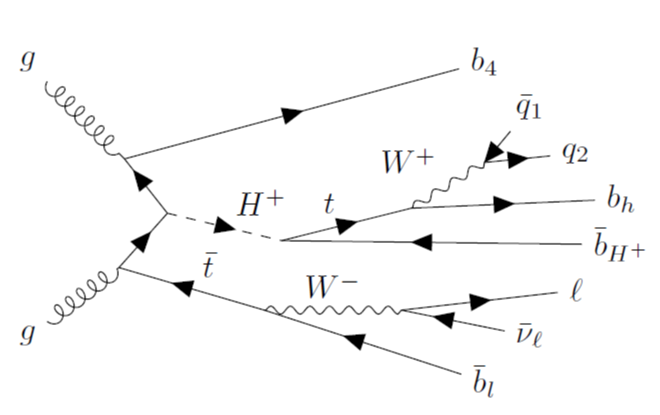
\includegraphics[keepaspectratio,scale=0.5]{images/AnalysisStrategy/FeynmanDiagram_Htb.png}
    \label{fig:FeynmanDiagram_Htb}
  }
  \subfloat[]{
    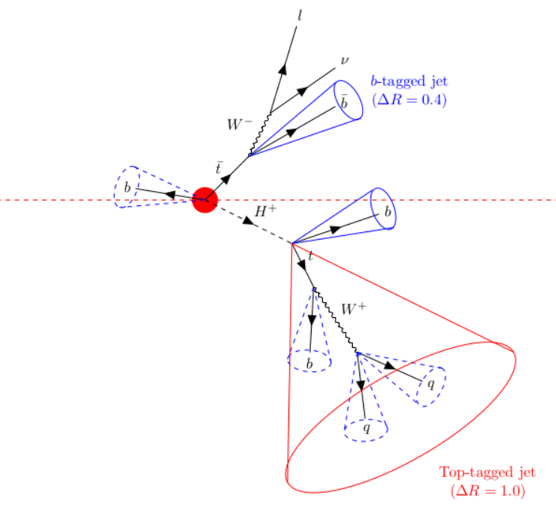
\includegraphics[keepaspectratio,scale=0.5]{images/AnalysisStrategy/EventTopology.png}
    \label{fig:EventTopology_Htb}
  }
  \caption{Feynman diagram (a) and schematic of boosted event topology (b). Signal event has at least one $J_{\text{top-tag}}$ and at least two $b$-tagged small-$R$ jets.}
  \label{fig:Diagram_Htb}
\end{figure}

To be consistent with the signal event as shown in Figure \ref{fig:Diagram_Htb}, events are required to have exactly one lepton ($e$ or ${\mu}$) that is matched to the one firing one of the single lepton triggers. Events are also required to have at least one top-tagged large-$R$ jet and at least two $b$-tagged small-$R$ jets. The $b$-jets must additionally satisfy ${\Delta}R(J_{\text{top-tag}}^{1st}, b\text{-jet})>1.0$ to ensure these $b$-jets are not consituent of the leading top-tagged jet.  These selections are summarized in Table \ref{tab:EventSelectionInSR}. 

\begin{table}[H]
  \centering
  \begin{tabular*}{150mm}{lll}
    \hline\hline
    \multicolumn{1}{c}{Cut} & \multicolumn{2}{c}{Criteria}\\
    \hline
    leptons                   & \multicolumn{2}{c}{\textbf{Exactly 1 lepton in event}}\\
                              & \underline{Electron}                & \underline{Muon}\\
                              & $p_{\text{T}}>27$ GeV               & $p_{\text{T}}>27$ GeV\\
                              & $|\eta|<1.37$ or $1.52<|\eta|<2.47$ & $|\eta|<2.5$\\
    \hline
    Top-tagged large-$R$ jets & \multicolumn{2}{c}{\textbf{${\geq}1$ top-tagged large-$R$ jets}}\\
                              & \multicolumn{2}{l}{$350~\text{GeV}<p_{\text{T}}<2500~\text{GeV}$}\\
                              & \multicolumn{2}{l}{$|\eta|<2.0$}\\
    \hline
    $b$-tagged small-$R$ jets & \multicolumn{2}{c}{\textbf{${\geq}2$ $b$-tagged small-$R$ jets}}\\
                              & \multicolumn{2}{l}{$p_{\text{T}}>25$ GeV}\\
                              & \multicolumn{2}{l}{$|\eta|<2.5$}\\
                              & \multicolumn{2}{l}{${\Delta}R(J_{\text{top-tag}}^{1st}, b\text{-jet})>1.0$}\\
    \hline\hline
  \end{tabular*}
  \caption{Event selections in the SR.}
  \label{tab:EventSelectionInSR}
\end{table}

Events passing the event selections in Table~\ref{tab:EventSelectionInSR} are expected to have the boosted-topology as shown in Figure \ref{fig:Diagram_Htb}.
The expected background composition and distributions in the SR is illustrated in Figure \ref{fig:BkgComposition_SR}. Events containing $t\bar{t}$ fully dominate the SR.
In this figure, $H_\text{T}^\text{jet}$ denotes the sum of $p_{\text{T}}$ of $J_\text{top-tag}^\text{1st}$ and all small-$R$ jets in event, and enhances the charasteristics of the signal events which have high $p_\text{T}$ jets from the heavy $H^+$ decay.

\begin{figure}[H]
  \centering
  \subfloat[]{
    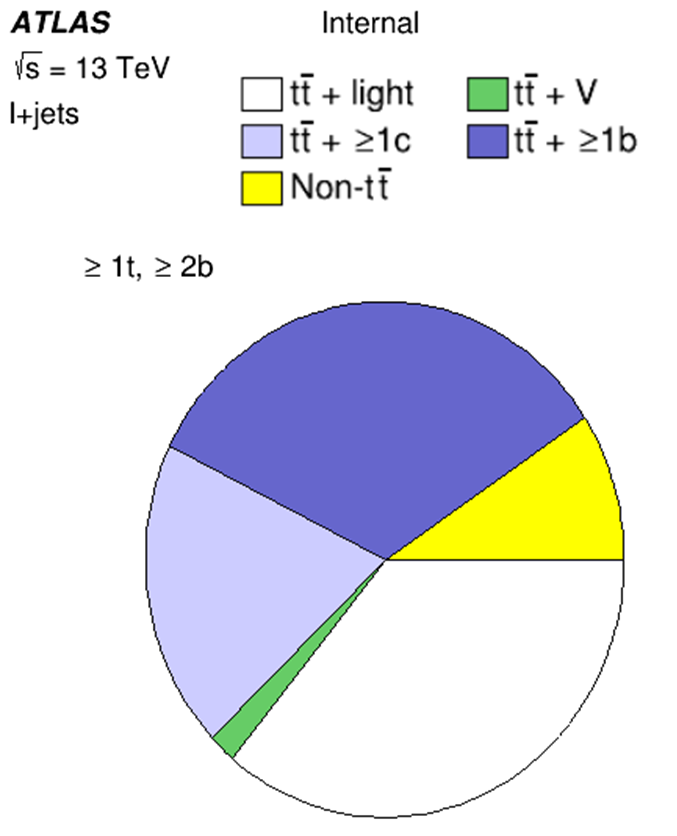
\includegraphics[keepaspectratio,scale=0.5]{images/AnalysisStrategy/PieChart_SR.png}
    \label{fig:PieChart_SR}
  }
  \subfloat[]{
    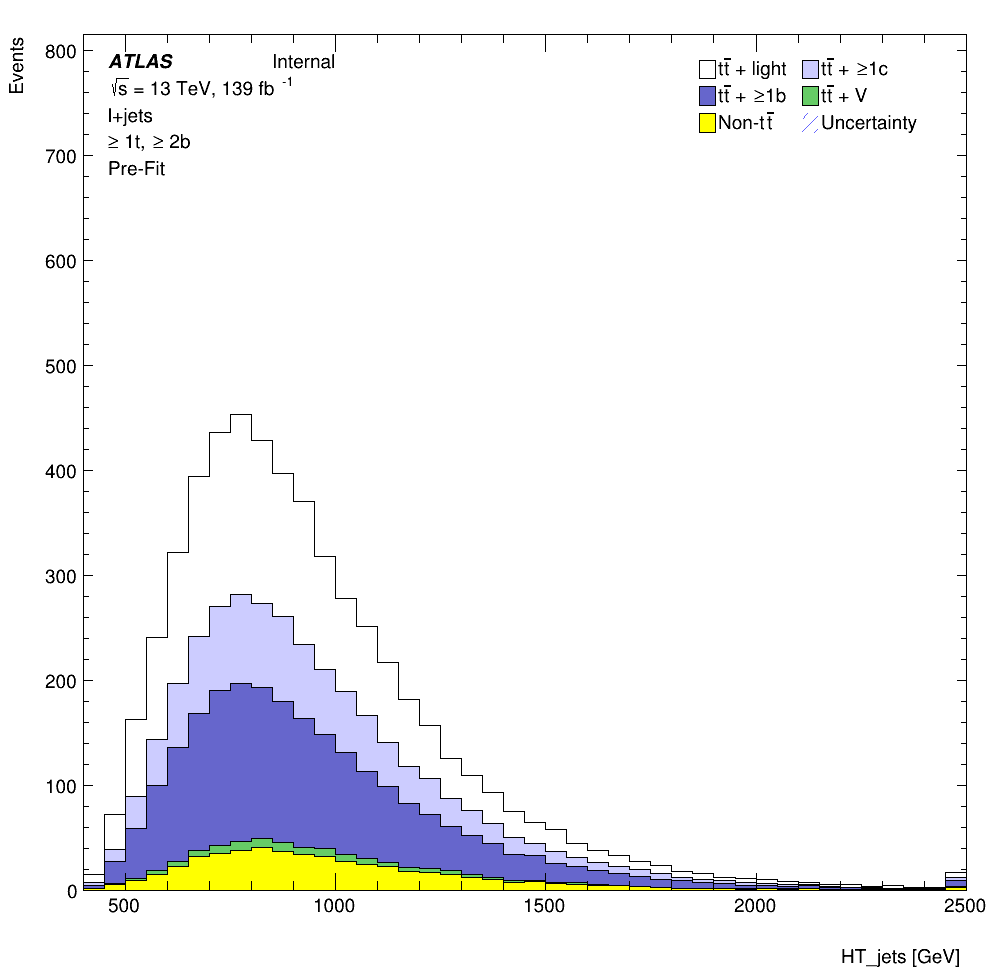
\includegraphics[keepaspectratio,scale=0.2]{images/AnalysisStrategy/HT_jets_SR.png}
    \label{fig:HT_jets_SR}
  }
  \caption{Background composition in the SR is shown in the pie chart (a) and the $H_{\text{T}}^{\text{jets}}$ distributions (b).}
  \label{fig:BkgComposition_SR}
\end{figure}




\subsubsection{Control region (CR)}
\label{subsec:EventSelection_CR}
In order to constrain the yields of events with $t\bar{t}$ in association with at least one light-flavor jet, a dedicated control region (CR) is prepared.
Requrements in the CR are identical to that in the SR, except the number of $b$-tagged small-$R$ jets. Exactrly one $b$-tagged small-$R$ jet is requred in the CR in order to keep orthogonality to the SR where two or more $b$-tagged small-$R$ jets are required. The selections in the CR are summarized in Table \ref{tab:EventSelectionInCR}. 

\begin{table}[H]
  \centering
  \begin{tabular*}{150mm}{ll}
    \hline\hline
    \multicolumn{1}{c}{Cut}   & \multicolumn{1}{c}{Criteria}\\
    \hline
    leptons                   & \multicolumn{1}{l}{Same as in the SR}\\
    \hline
    Top-tagged large-$R$ jets & \multicolumn{1}{l}{Same as in the SR}\\
    \hline
    $b$-tagged small-$R$ jets & \multicolumn{1}{l}{Exactly one $b$-tagged small-$R$ jet}\\
                              & \multicolumn{1}{l}{Other kinematic requrements are the same as in the SR}\\
    \hline\hline
  \end{tabular*}
  \caption{Event selections in the CR.}
  \label{tab:EventSelectionInCR}
\end{table}

After applying the event selections for the CR, the events mostly contain $t\bar{t}$ in association with at least one light-flavor jet. The background composition is illustrated in Figure \ref{fig:BkgComposition_CR}. 
This CR is included in the profile likelihood fit discussed in Section \ref{sec:ProfileLikelohoodFit}. 

\begin{figure}[H]
  \centering
  \subfloat[]{
    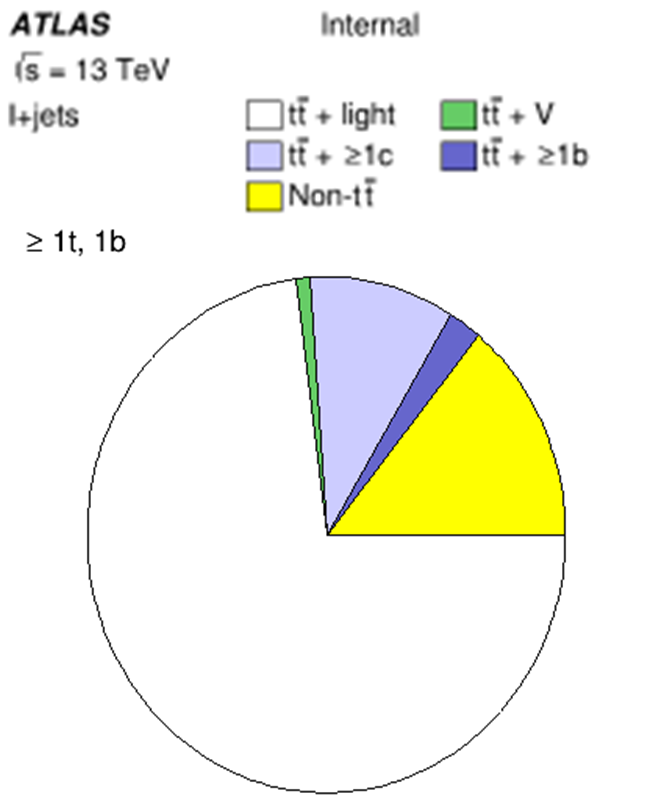
\includegraphics[keepaspectratio,scale=0.5]{images/AnalysisStrategy/PieChart_CR.png}
    \label{fig:PieChart_CR}
  }
  \subfloat[]{
    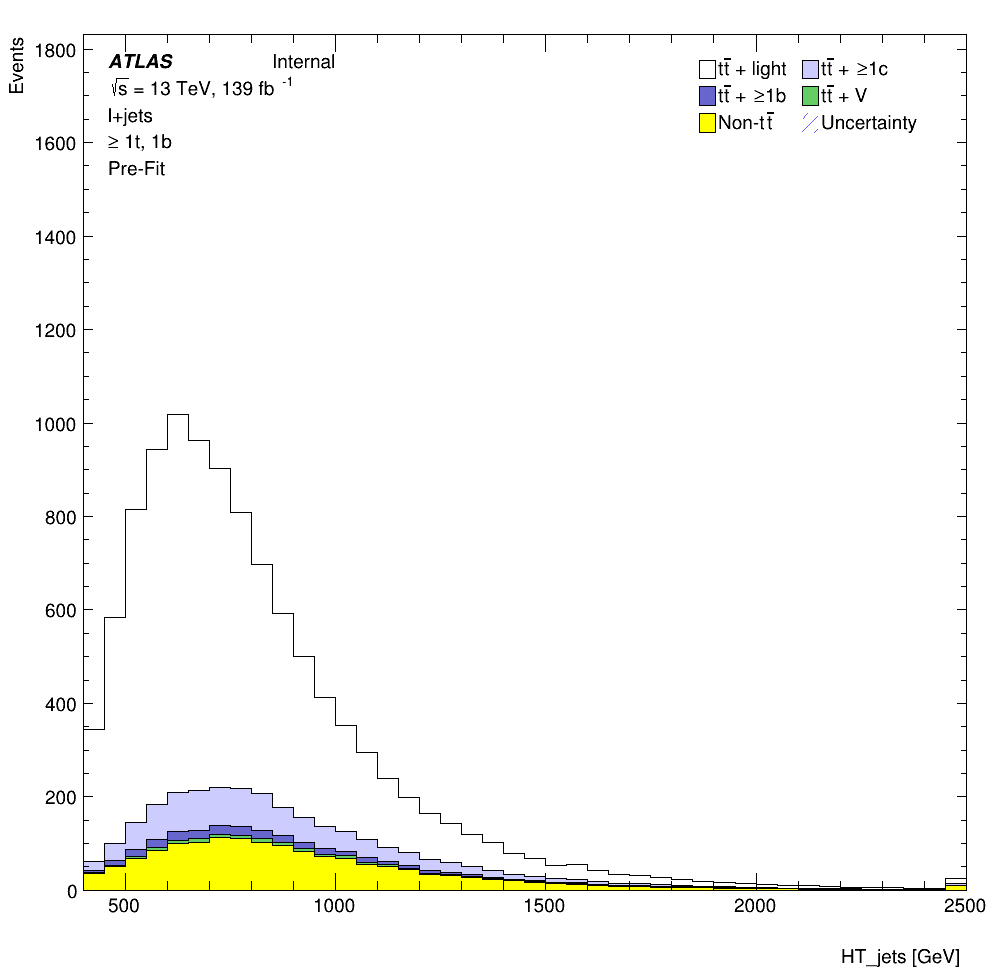
\includegraphics[keepaspectratio,scale=0.2]{images/AnalysisStrategy/HT_jets_CR.png}
    \label{fig:HT_jets_CR}
  }
  \caption{Background composition in the CR is shown in the pie chart (a) and the $H_{\text{T}}^{\text{jets}}$ distributions (b).}
  \label{fig:BkgComposition_CR}
\end{figure}




\subsubsection{Summary}
The number of expected signal and background events in the SR and CR are shown in Table \ref{tab:PrefitYields}. The predicted number of $H^{+}$ signal events for the 1000 and 3000 GeV mass hypothesis assume ${\sigma}{\times}Br=0.046$~pb. This is the upper limit at $M_{H^{+}}=1000$~GeV obtained from the resolved analysis.

\begin{table}[H]
  \centering
  \begin{tabular*}{150mm}{@{\extracolsep{\fill}}cll}
    \hline\hline
                            & \multicolumn{1}{c}{SR} & \multicolumn{1}{c}{CR}\\
    \hline
    $t\bar{t}+\text{light}$ & $1979\pm 89$           & $ 7848\pm329$ \\
    $t\bar{t}+\geq1c$       & $1070\pm 56$           & $ 1052\pm 38$ \\
    $t\bar{t}+\geq1b$       & $1840\pm 84$           & $  246\pm 11$ \\
    $t\bar{t}+W$            & $  38\pm 20$           & $   52\pm 27$ \\
    $t\bar{t}+Z$            & $  67\pm 34$           & $   49\pm  6$ \\
    $Wt$ channel            & $ 183\pm 93$           & $  422\pm212$ \\
    $t$ channel             & $  37\pm  3$           & $   63\pm  5$ \\
    Other top sources       & $  38\pm 15$           & $   11\pm  1$ \\
    $VV$, $V$+jets          & $ 152\pm 55$           & $ 1001\pm342$ \\
    $t\bar{t}H$             & $ 103\pm  4$           & $   18\pm  0$ \\
    \hline
    Total                   & $5565\pm256$           & $10763\pm566$ \\
    \hline
    $H^{+}$ 1000 GeV        & $  58\pm  6$           & $    4\pm  0$ \\
    $H^{+}$ 3000 GeV        & $  67\pm 16$           & $   13\pm  3$ \\
    \hline\hline
  \end{tabular*}
  \caption{Number of expected and selected events split according to the analysis region. The quated uncertainties include both statistical and systematic uncertainties before fitting.}
  \label{tab:PrefitYields}
\end{table}

\subsection{Multivariable analysis using BDT}
\label{subsec:MVA}
In this search, the most important background is $t\bar{t}+\text{jets}$ as discussed in Section \ref{subsec:EventSelection_SR}. To enhance separation between signal and background, multivariable analysis is performed using Boosted Decision Trees (BDT) technique. Obtained BDT score distribution is used in the profile likelihood fit as a final discriminant (Section \ref{sec:ProfileLikelohoodFit}).

\subsubsection{Signal and background definition in BDT training}
To classify $H^{+}$ signal and $t\bar{t}+\text{jets}$ background events, BDTs are trained using the simucalted $H^{+}$ signal and $t\bar{t}+\text{jets}$ background samples, as summarized in Table~\ref{tab:BDTInputDatasets}. Ten different $H^{+}$ mass hypotheses are considered in this analysis, and the training is performed on each $H^{+}$ mass hypothesis. On the other hand, the $t\bar{t}+\text{jets}$ background samples are common in each training. Since kinematics of $H^+$ signals become harder in higher mass hypotheses, as shown in Section~\ref{subsubsec:BDTInputVars}, the BDTs trained using the higher $H^{+}$ mass samples typically have greater separation power.

\begin{table}[H]
  \centering
  \begin{tabular*}{140mm}{c|c|c}
    \hline
    $H^{+}$ mass  point  & DSID (Signal sample) & DSID (Background sample)\\
    \hline
    $M_{H^{+}}=$1000 GeV & 450004               & \\
    $M_{H^{+}}=$1200 GeV & 450598               & \textbf{$t\bar{t}+\text{jets}$ (Inclusive):}\\
    $M_{H^{+}}=$1400 GeV & 450599               & [410470, 410471]\\
    $M_{H^{+}}=$1600 GeV & 450600               & \textbf{$t\bar{t}+\text{jets}$ (BBFilter):}\\
    $M_{H^{+}}=$1800 GeV & 450601               & [411073, 411076]\\
    $M_{H^{+}}=$2000 GeV & 450602               & \textbf{$t\bar{t}+\text{jets}$ (BFilterBBVeto):}\\
    $M_{H^{+}}=$2500 GeV & 451490               & [411074,411077]\\
    $M_{H^{+}}=$3000 GeV & 451491               & \textbf{$t\bar{t}+\text{jets}$ (CFilterBVeto):}\\
    $M_{H^{+}}=$4000 GeV & 508710               & [411075,411078]\\
    $M_{H^{+}}=$5000 GeV & 508711               & \\
    \hline
  \end{tabular*}
  \caption{Signal and background samples used for BDT training.}
  \label{tab:BDTInputDatasets}
\end{table}

\subsubsection{BDT training settings}
\label{subsubsec:BDTTrainingSettings}
In order to make full use of statistics of simulation samples, 4-fold cross-validation is used. Each simulation sample is divided into four sub-datasets at random by a seed value based on the MC event number, and labeled by ``TRAIN'', ``VALID'' and ``TEST''. Two of the four sub-datasets are assigned ``TRAIN'', which are used for BDT training. One of the other sub-datasets are assigend ``VALID'', and is used to optimize the BDT performance. The last sample, ``TEST'' is used to construct a fit template. There are four possible combinations for sub-division of the samples as shown in Figure \ref{fig:CrossValidationScheme}. The four statistically-independent BDTs are obtained from the four ``TEST'' sub-datasets, and they are combined into one fit template, which is used in the profile likelihood fit (Section. \ref{sec:ProfileLikelohoodFit}).

\begin{figure}[H]
  \centering
  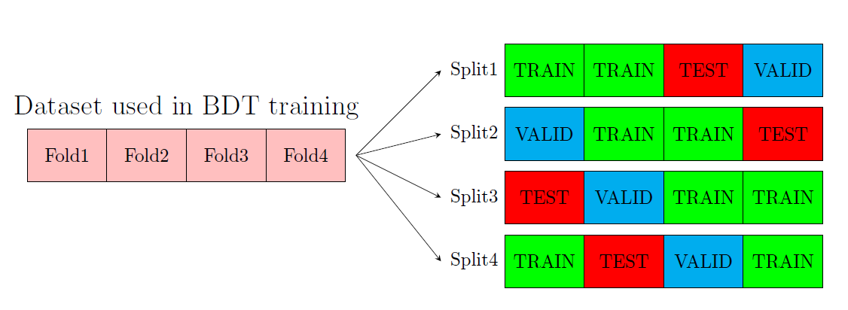
\includegraphics[keepaspectratio,scale=0.50]{images/AnalysisStrategy/CrossValidationScheme.png}
  \caption{Scheme of 4-fold cross-validation in this analysis.}
  \label{fig:CrossValidationScheme}
\end{figure}

Hyperparamerters for the BDTs are summarized in Table. \ref{tab:Hyperparameters}. Those hyperparameters are chosen to obtain the best sensitivity.
    
\begin{table}[H]
  \centering
  \begin{tabular*}{75mm}{@{\extracolsep{\fill}}ll}
    \hline
    \multicolumn{1}{c}{Configuration} & \multicolumn{1}{c}{}\\
    \hline\hline
    \multicolumn{1}{l}{Algorithm}     & \multicolumn{1}{c}{Gradient boosting}\\
    \hline
    $Hyperparameters$ & \\
    \multicolumn{1}{l}{NTrees}       & \multicolumn{1}{c}{100}\\
    \multicolumn{1}{l}{MinNodeSize}  & \multicolumn{1}{c}{2.5}\\
    \multicolumn{1}{l}{MaxDepth}     & \multicolumn{1}{c}{3}\\
    \multicolumn{1}{l}{nCuts}        & \multicolumn{1}{c}{20}\\
    \hline
  \end{tabular*}
  \caption{List of hyperparameters used in the trainging of a BDT}
  \label{tab:Hyperparameters}
\end{table}
    
\subsubsection{Input variables in BDT}
\label{subsubsec:BDTInputVars}
Jets originating from an $H^{+}$ decay have higher $p_\text{T}$ comparing with $t\bar{t}+\text{jets}$ events due to its heavy mass. Additionally, correlation among jets are different between $H^{+}$ and $t\bar{t}+\text{jets}$ events because $H^+$ creates a resonance. The BDT is trained in order to fully exploit these kinematic characteristics. List of variables used in BDT training is summarized in Table \ref{tab:BDTInputVariables}. In Figure \ref{fig:SOVERB_Hp3000_Contained80_DL1r_70}, each distribution in the $H^{+}$ sample with a mass of 3000~GeV is compared with the $t\bar{t}+\text{jets}$ background. 

\begin{table}[H]
  \centering
  \begin{tabular*}{150mm}{@{\extracolsep{\fill}}ll}
    \hline
    \multicolumn{1}{c}{Symbol} & \multicolumn{1}{c}{Description}\\
    \hline\hline
    HT\_jets                                   & Scalar sum of the transverse energy of all jets\\
    LeadingJet\_pt                             & Leading jet $p_\text{T}$\\
    Mjjj\_MaxPt                                & Invariant mass of the jet triplet with maximum $p_\text{T}$\\
    Mbb\_MaxPt                                 & Invariant mass of the b-jet pair with maximum $p_\text{T}$\\
    Muu\_MindR                                 & Invariant mass of the untagged jet-pair with minimum $\Delta{R}$\\
    dRlepbb\_MindR                             & $\Delta{R}$ between the lepton and the pair of $b$-jets with smallest $\Delta{R}$\\
    dRbb\_avg                                  & Average $\Delta{R}$ between all $b$-jet pairs in the event\\
    Centrality\_all                            & Centrality calculated using all jets and leptons\\
    H1\_all                                    & Second Fox-Wolfram moment calculated using all jets and leptons\\
    LeadingTop\_pt                             & Leading top-tagged jet $p_\text{T}$\\
    LeadingTop\_m                              & Invariant mass of leading top-tagged jet \\
    Pt\_tb                                     & $p_\text{T}$ of the pair of leading top-tagged jet and leading $b$-jet\\
    M\_tb                                      & Invariant mass of the pair of leading top-tagged jet and leading $b$-jet\\
    PtAsymm\_tb                                & $p_\text{T}$ asymmetry between leading top-tagged jet and leading $b$-jet\\
    \hline
  \end{tabular*}
  \caption{List of variables included in the training of the BDT}
  \label{tab:BDTInputVariables}
\end{table}

\begin{figure}[H]
  \subfloat[HT\_jets] {
    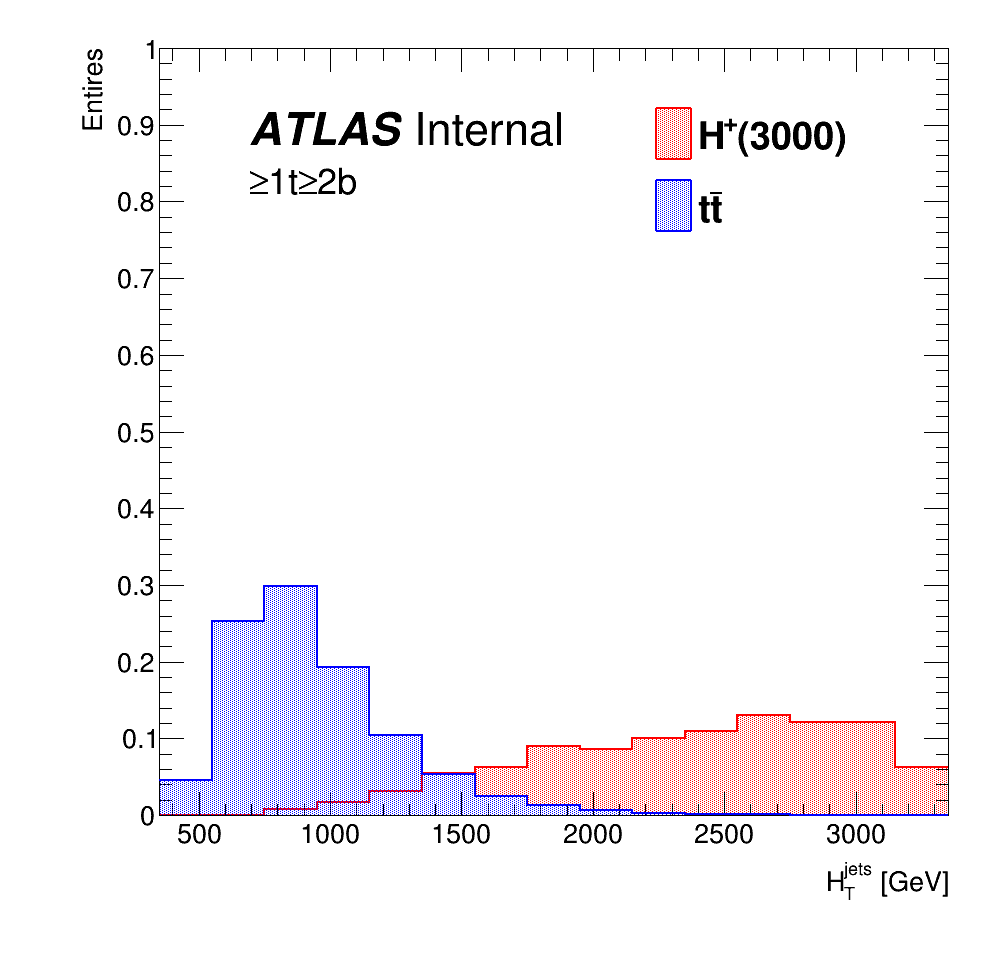
\includegraphics[width=0.25\textwidth]{images/AnalysisStrategy/SOVERB_Hp3000_Contained80_DL1r_70_HT_jets_Contained80_DL1r_70.png}
    \label{fig:SOVERB_HT_jets_Hp3000_Contained80_DL1r_70}    
  }
  \subfloat[LeadingJet\_pt] {
    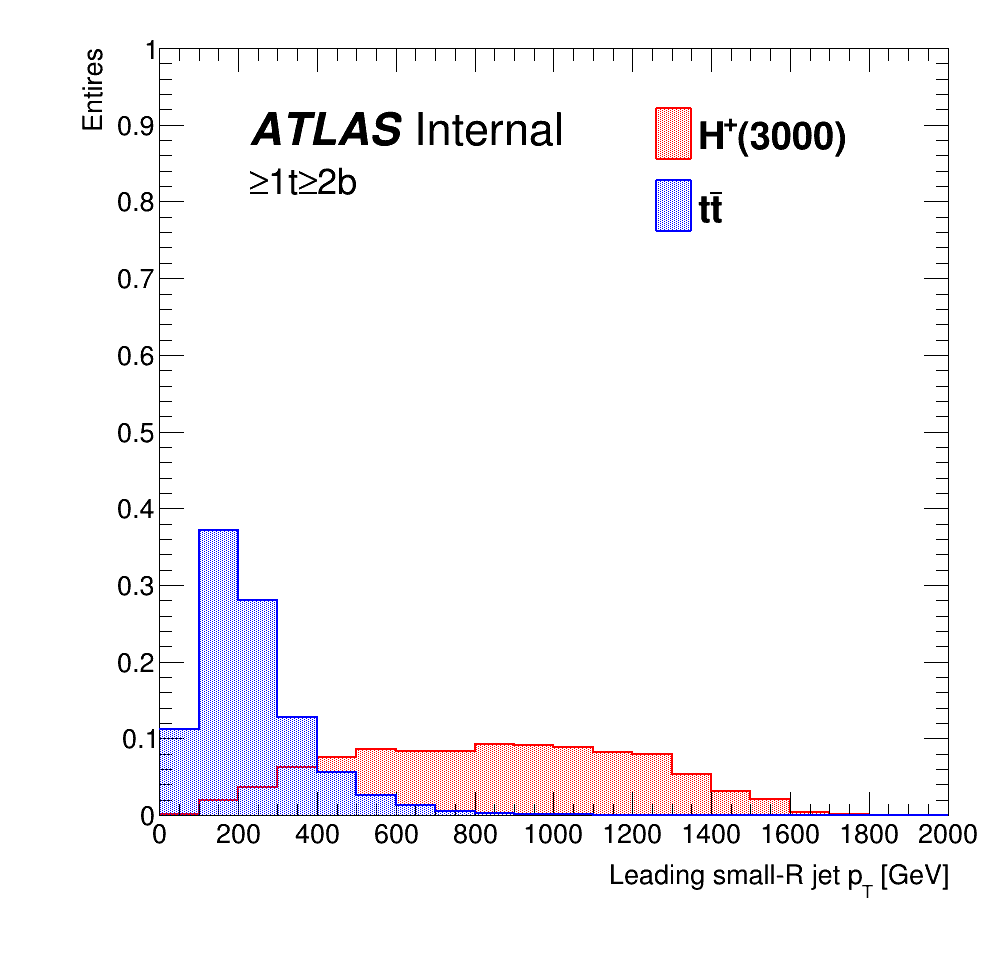
\includegraphics[width=0.25\textwidth]{images/AnalysisStrategy/SOVERB_Hp3000_Contained80_DL1r_70_leadingJet_pt_Contained80_DL1r_70.png}
    \label{fig:SOVERB_LeadingJet_pt_Hp3000_Contained80_DL1r_70}    
  }
  \subfloat[Centrality\_all] {
    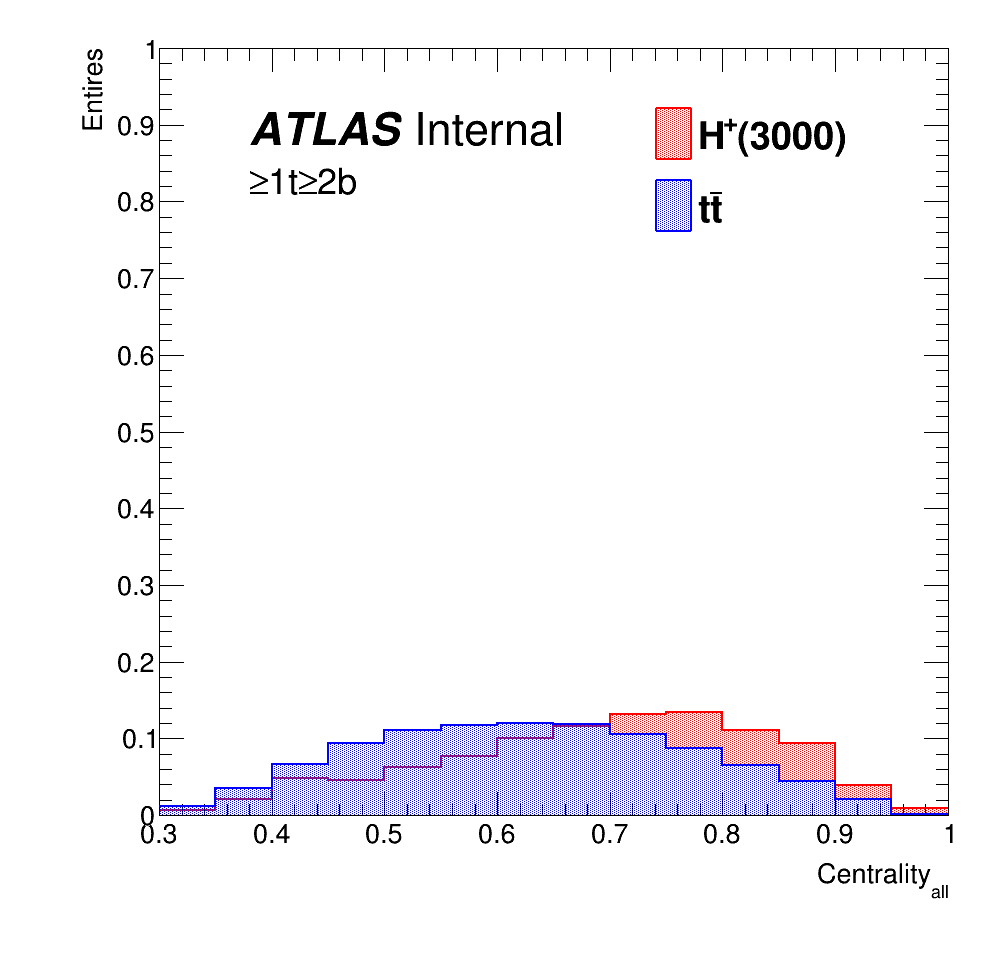
\includegraphics[width=0.25\textwidth]{images/AnalysisStrategy/SOVERB_Hp3000_Contained80_DL1r_70_Centrality_all_Contained80_DL1r_70.png}
    \label{fig:SOVERB_Centrality_all_Hp3000_Contained80_DL1r_70}    
  }
  \subfloat[H1\_all] {
    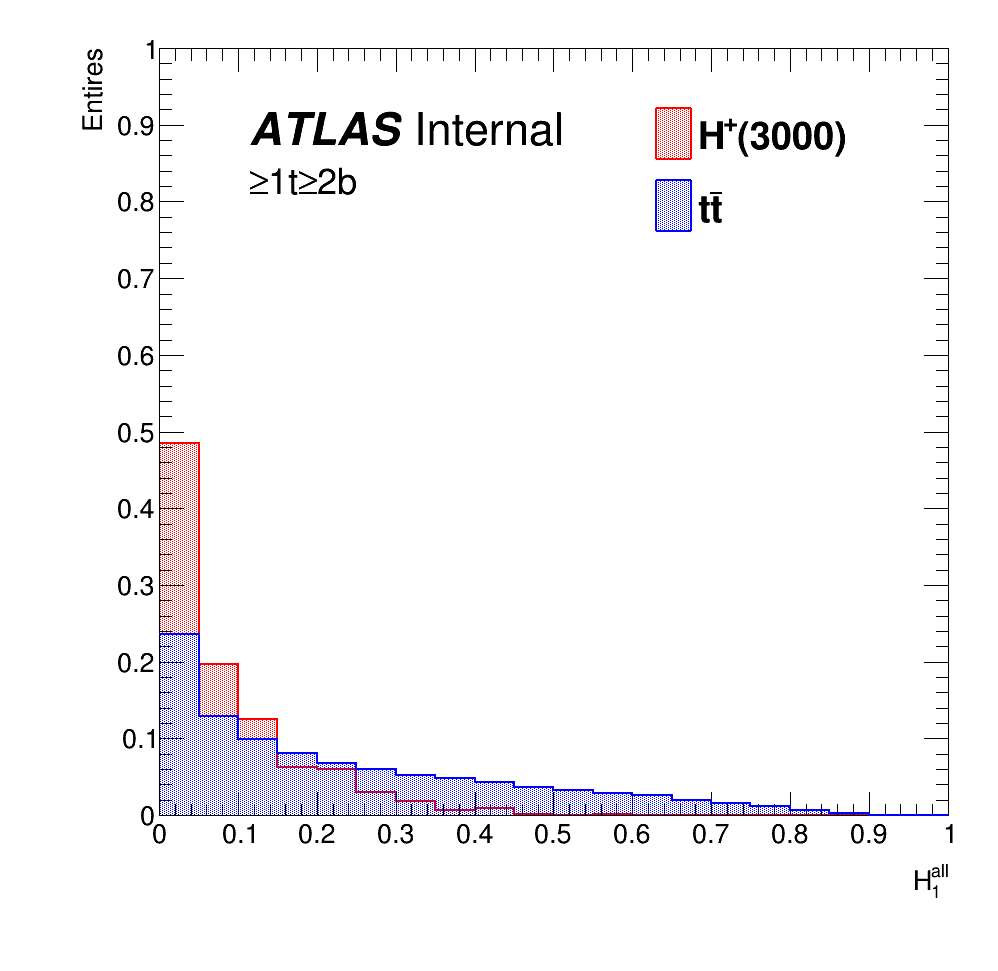
\includegraphics[width=0.25\textwidth]{images/AnalysisStrategy/SOVERB_Hp3000_Contained80_DL1r_70_H1_all_Contained80_DL1r_70.png}
    \label{fig:SOVERB_H1_all_Hp3000_Contained80_DL1r_70}    
  }\\
  \subfloat[Mbb\_MaxPt] {
    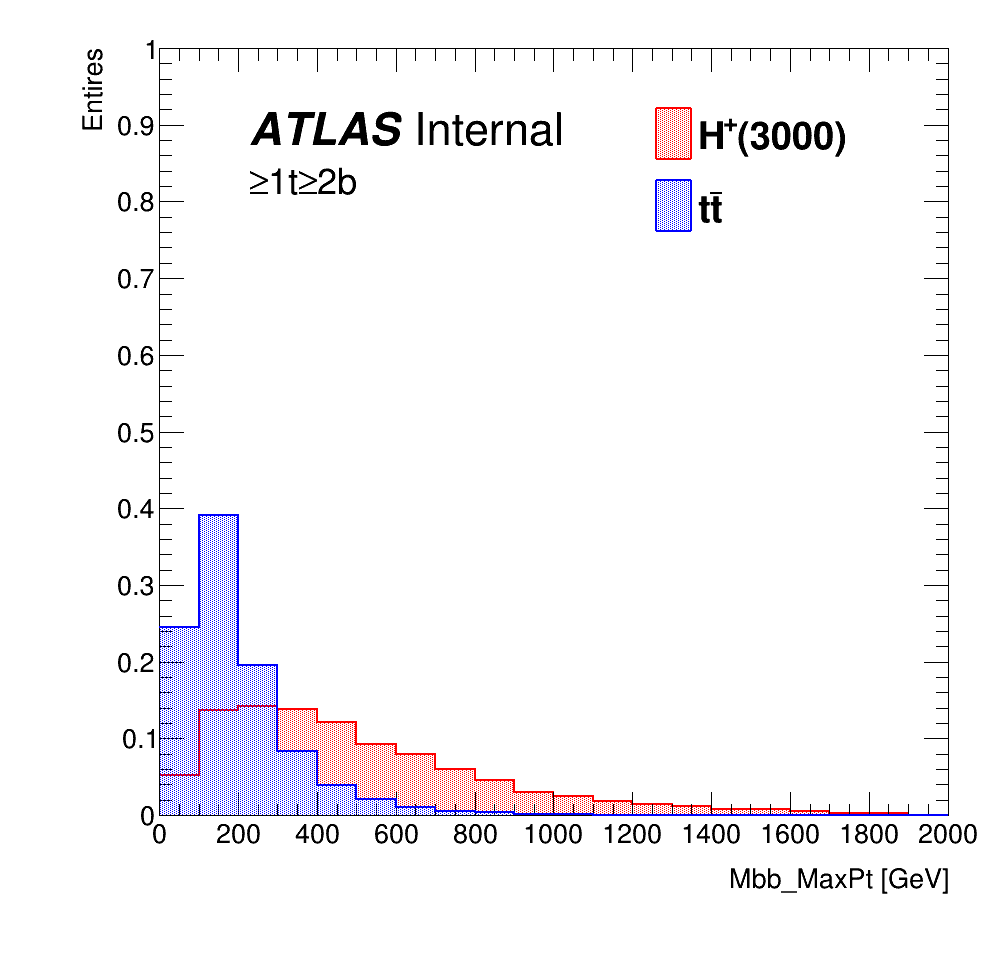
\includegraphics[width=0.25\textwidth]{images/AnalysisStrategy/SOVERB_Hp3000_Contained80_DL1r_70_Mbb_MaxPt_Contained80_DL1r_70.png}
    \label{fig:SOVERB_Mbb_MaxPt_Hp3000_Contained80_DL1r_70}    
  }
  \subfloat[Mjjj\_MaxPt] {
    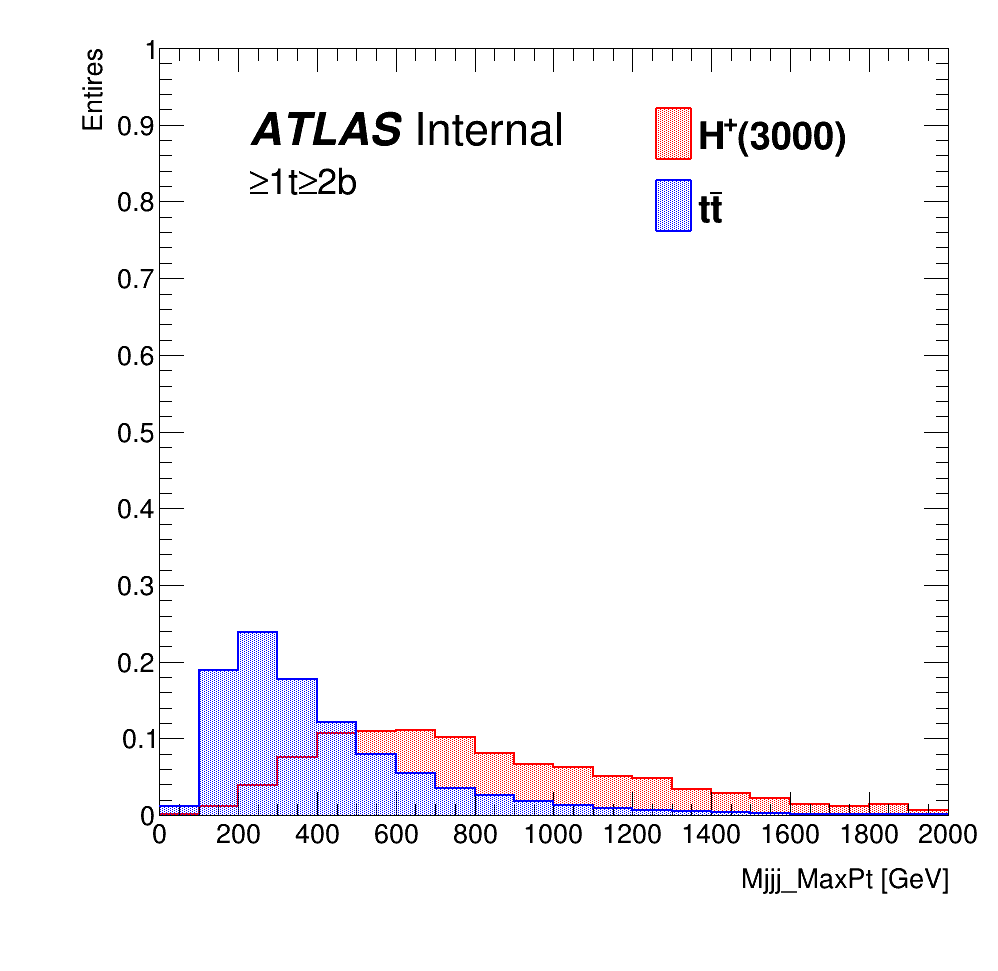
\includegraphics[width=0.25\textwidth]{images/AnalysisStrategy/SOVERB_Hp3000_Contained80_DL1r_70_Mjjj_MaxPt_Contained80_DL1r_70.png}
    \label{fig:SOVERB_Mjjj_MaxPt_Hp3000_Contained80_DL1r_70}    
  }
  \subfloat[Muu\_MindR] {
    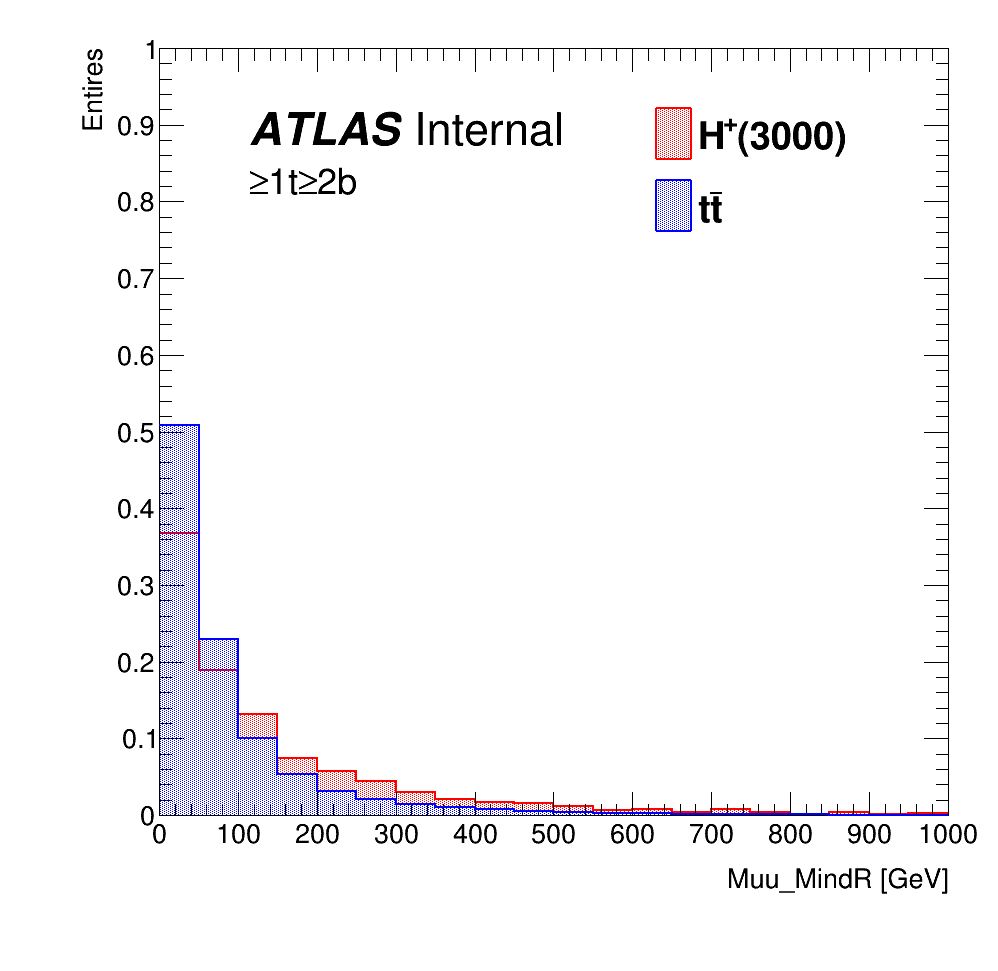
\includegraphics[width=0.25\textwidth]{images/AnalysisStrategy/SOVERB_Hp3000_Contained80_DL1r_70_Muu_MindR_Contained80_DL1r_70.png}
    \label{fig:SOVERB_Muu_MindR_Hp3000_Contained80_DL1r_70}    
  }
  \subfloat[dRbb\_avg] {
    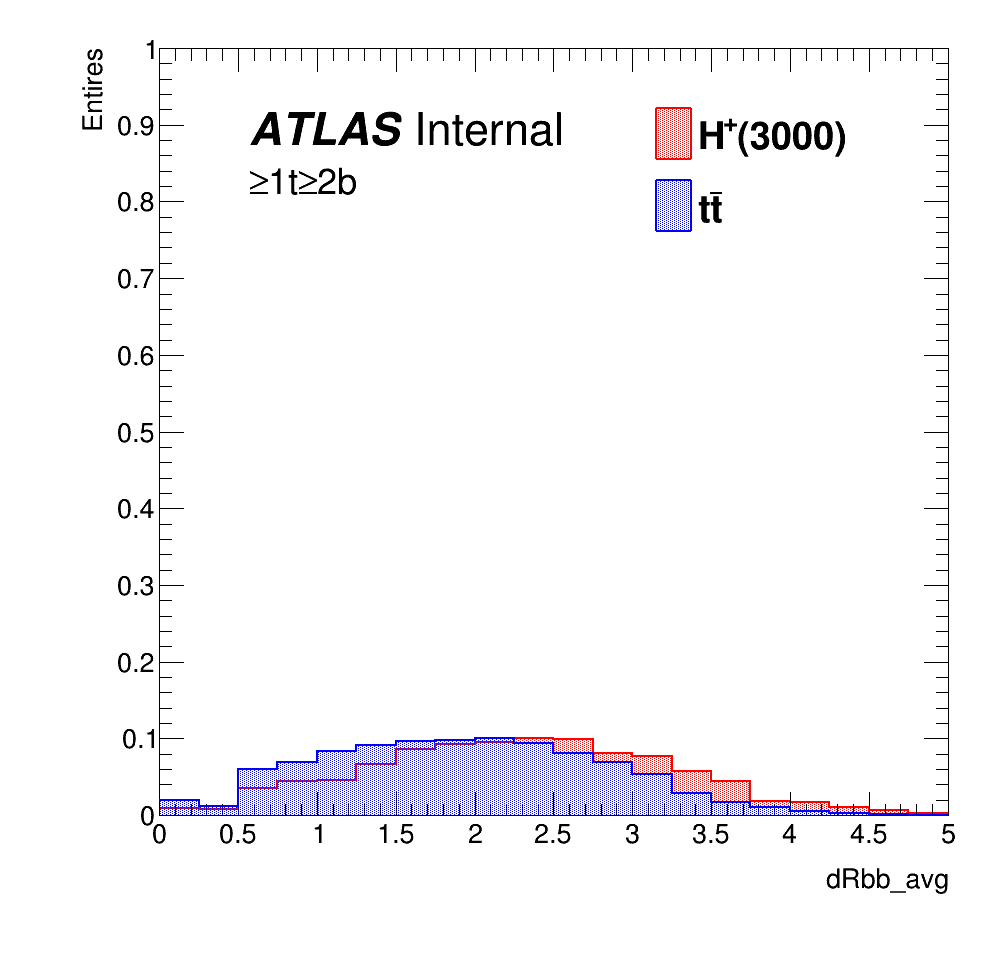
\includegraphics[width=0.25\textwidth]{images/AnalysisStrategy/SOVERB_Hp3000_Contained80_DL1r_70_dRbb_avg_Contained80_DL1r_70.png}
    \label{fig:SOVERB_dRbb_avg_Hp3000_Contained80_DL1r_70}    
  }\\
  \subfloat[dRlepbb\_MindR] {
    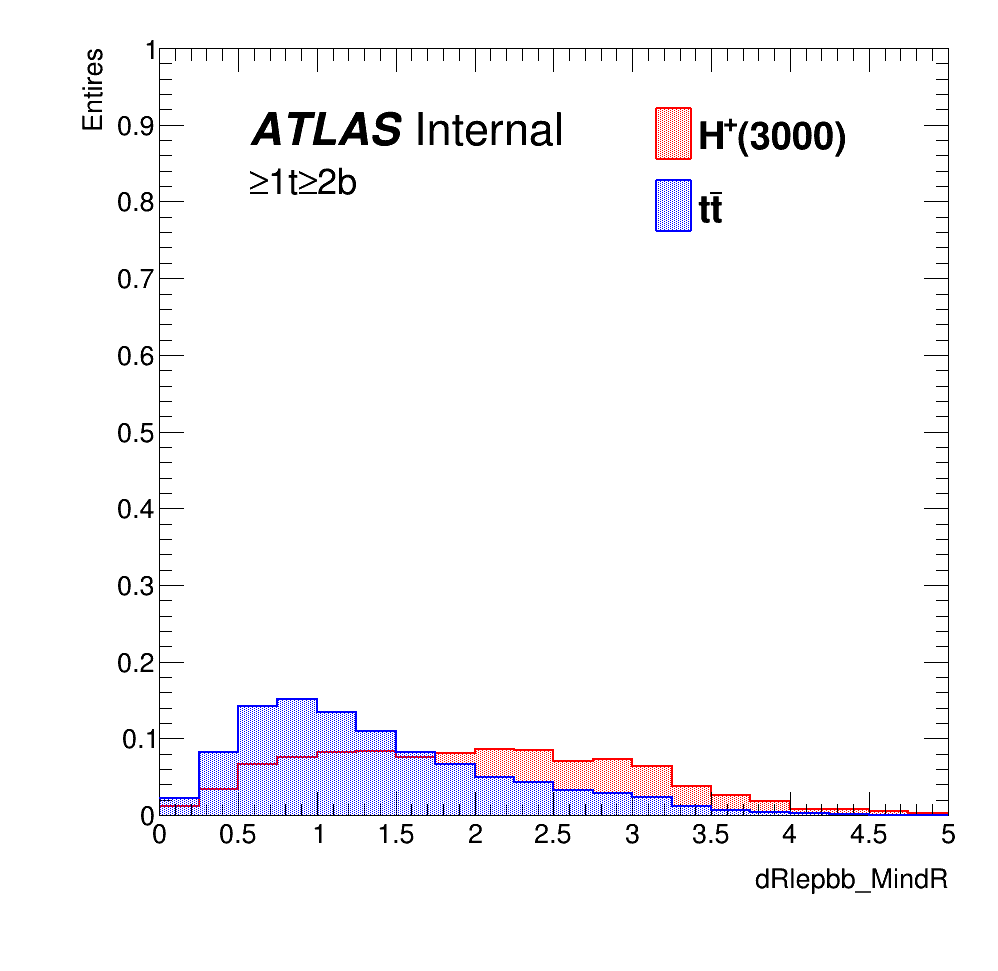
\includegraphics[width=0.25\textwidth]{images/AnalysisStrategy/SOVERB_Hp3000_Contained80_DL1r_70_dRlepbb_MindR_Contained80_DL1r_70.png}
    \label{fig:SOVERB_dRlepbb_MindR_Hp3000_Contained80_DL1r_70}    
  }
  \subfloat[LeadingTop\_m] {
    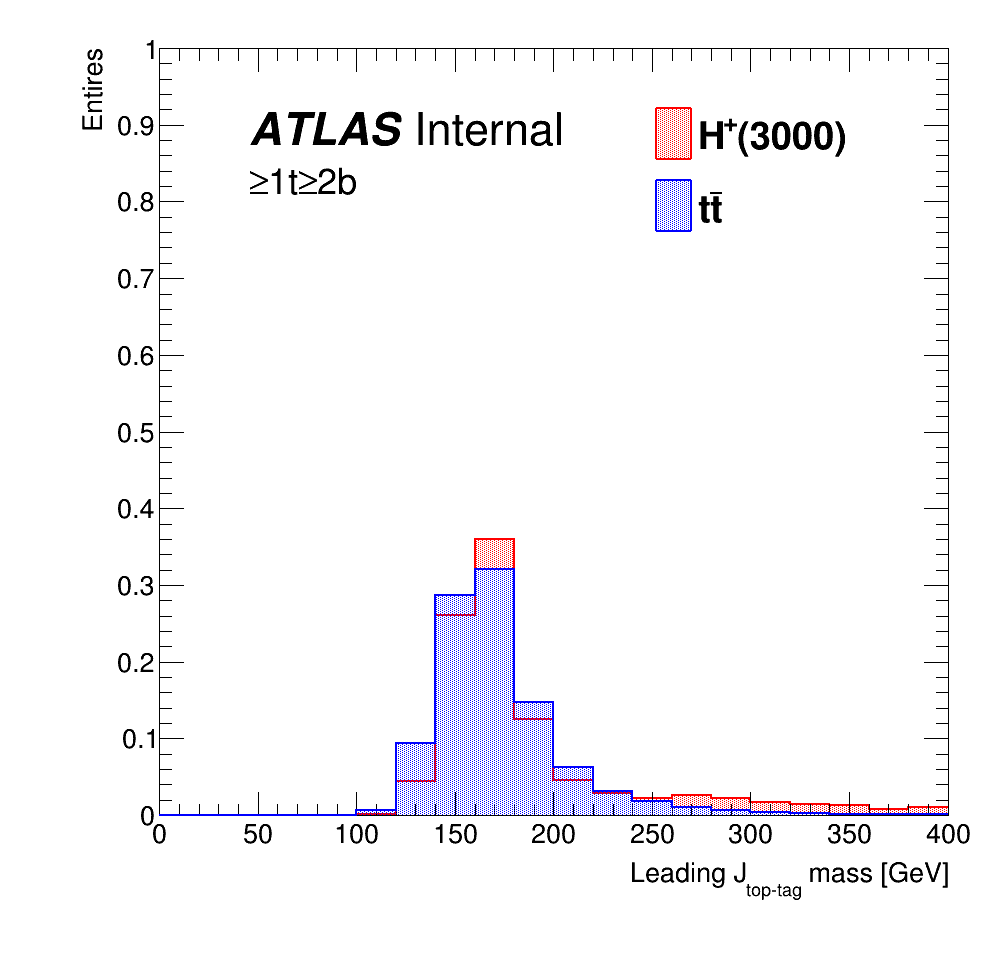
\includegraphics[width=0.25\textwidth]{images/AnalysisStrategy/SOVERB_Hp3000_Contained80_DL1r_70_leadingTop_m_Contained80_DL1r_70.png}
    \label{fig:SOVERB_leadingTop_mass_Hp3000_Contained80_DL1r_70}    
  }
  \subfloat[LeadingTop\_pt] {
    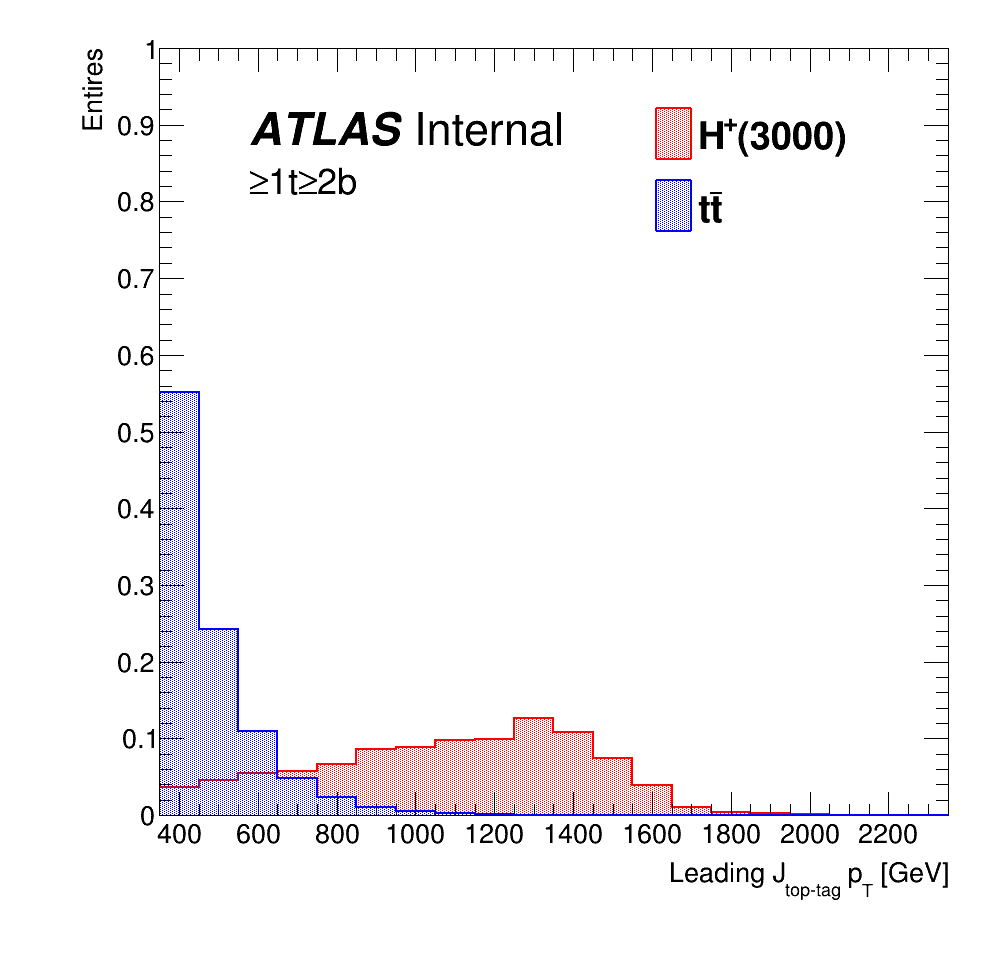
\includegraphics[width=0.25\textwidth]{images/AnalysisStrategy/SOVERB_Hp3000_Contained80_DL1r_70_leadingTop_pt_Contained80_DL1r_70.png}
    \label{fig:SOVERB_leadingTop_pt_Hp3000_Contained80_DL1r_70}    
  }
  \subfloat[M\_tb] {
    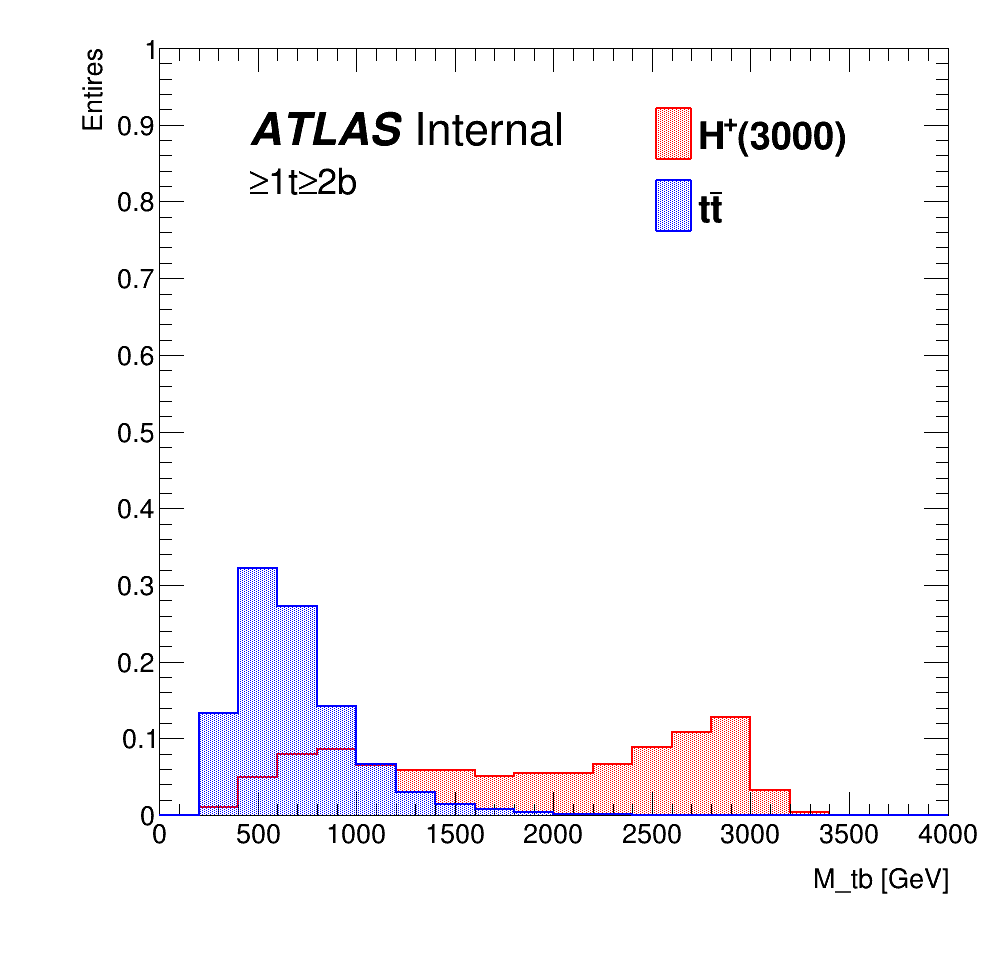
\includegraphics[width=0.25\textwidth]{images/AnalysisStrategy/SOVERB_Hp3000_Contained80_DL1r_70_tb_m_Contained80_DL1r_70.png}
    \label{fig:SOVERB_M_tb_Hp3000_Contained80_DL1r_70}    
  }\\
  \subfloat[Pt\_tb] {
    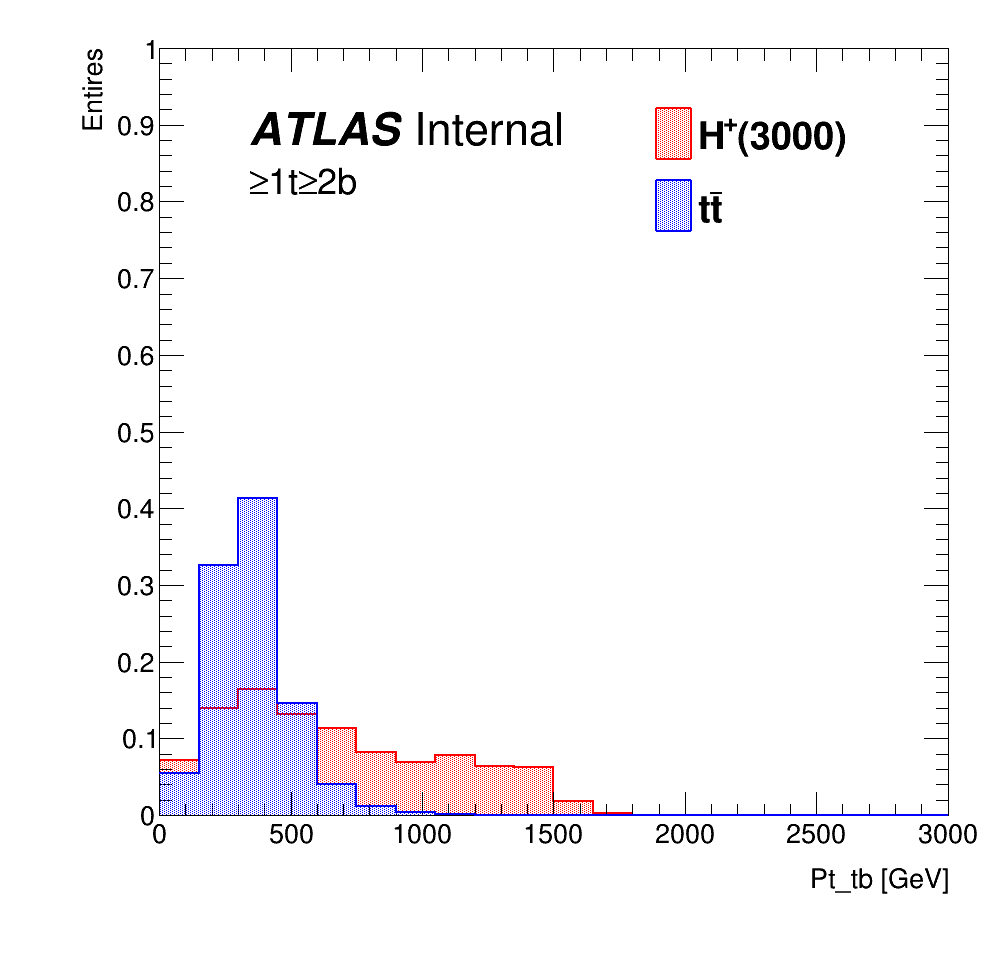
\includegraphics[width=0.25\textwidth]{images/AnalysisStrategy/SOVERB_Hp3000_Contained80_DL1r_70_tb_pt_Contained80_DL1r_70.png}
    \label{fig:SOVERB_Pt_tb_Hp3000_Contained80_DL1r_70}    
  }
  \subfloat[PtAsymm\_tb] {
    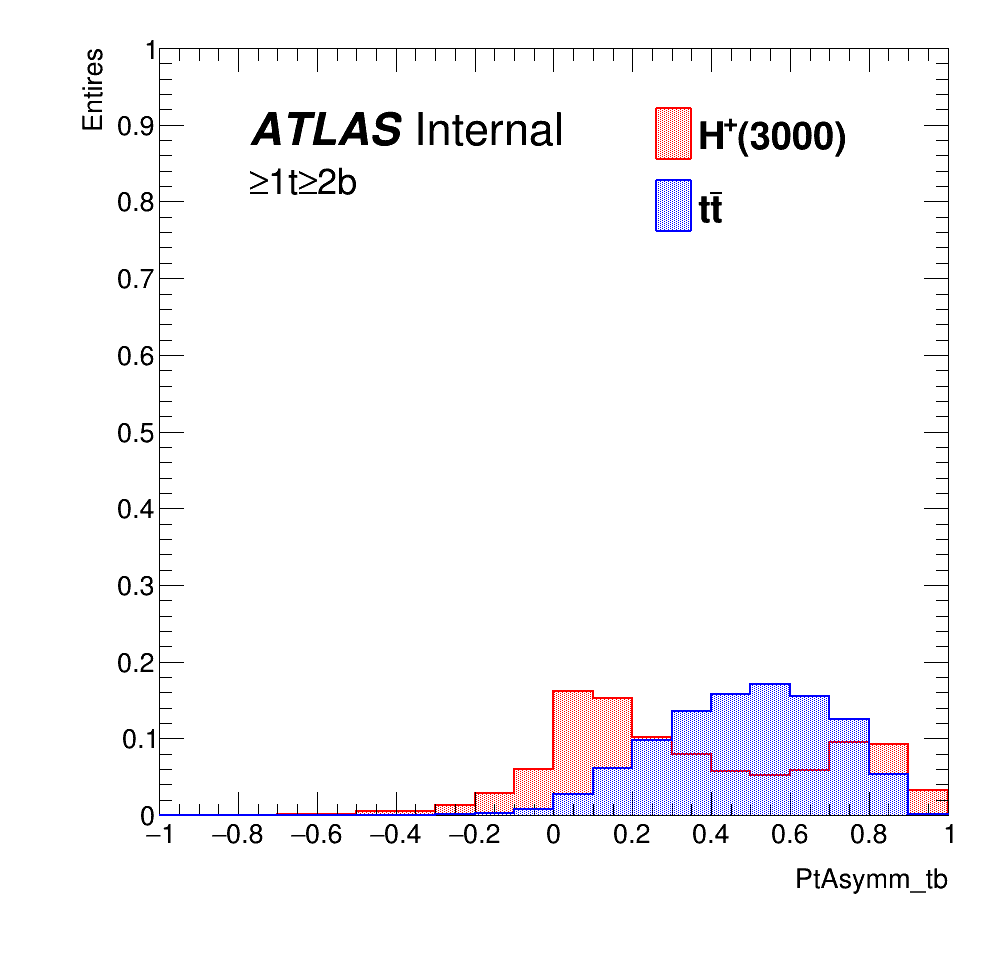
\includegraphics[width=0.25\textwidth]{images/AnalysisStrategy/SOVERB_Hp3000_Contained80_DL1r_70_tb_ptAsymm_Contained80_DL1r_70.png}
    \label{fig:SOVERB_PtAsymm_tb_Hp3000_Contained80_DL1r_70}    
  }
  
  \caption{Comparison of input variables for BDT training between $H^{+}$ and $t\bar{t}+\text{jets}$ events under 3000 GeV $H^{+}$ mass hypothesis.}
  \label{fig:SOVERB_Hp3000_Contained80_DL1r_70}    
\end{figure}

\subsubsection{Results of BDT training}
\label{subsubsec:ResultBDTTraingin}
The BDT output distributions for signal and background in the analysis region for different values of the $H^+$ mass are shown in Figure \ref{fig:BDTTrainingResults_Hp1000} to \ref{fig:BDTTrainingResults_Hp3000}, together with receiver operating charasteristic (ROC) curves.

%%% BDT trainging results for H+(1000)
\begin{figure}[H]
  \centering
  \subfloat[BDT output]{
    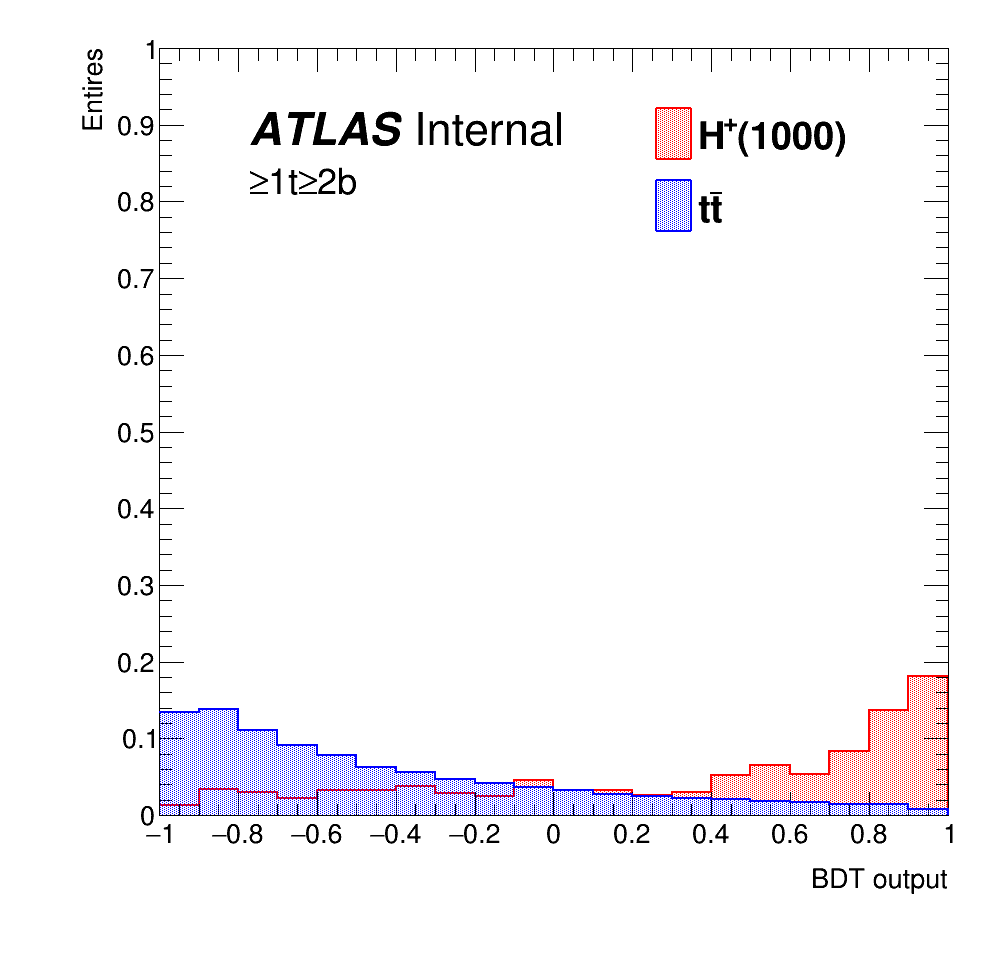
\includegraphics[width=0.45\textwidth]{images/AnalysisStrategy/BDTOutput_Hp1000_Contained80_DL1r_70.png}
    \label{fig:BDTOutput_Hp1000}
  }
  \subfloat[ROC curve]{
    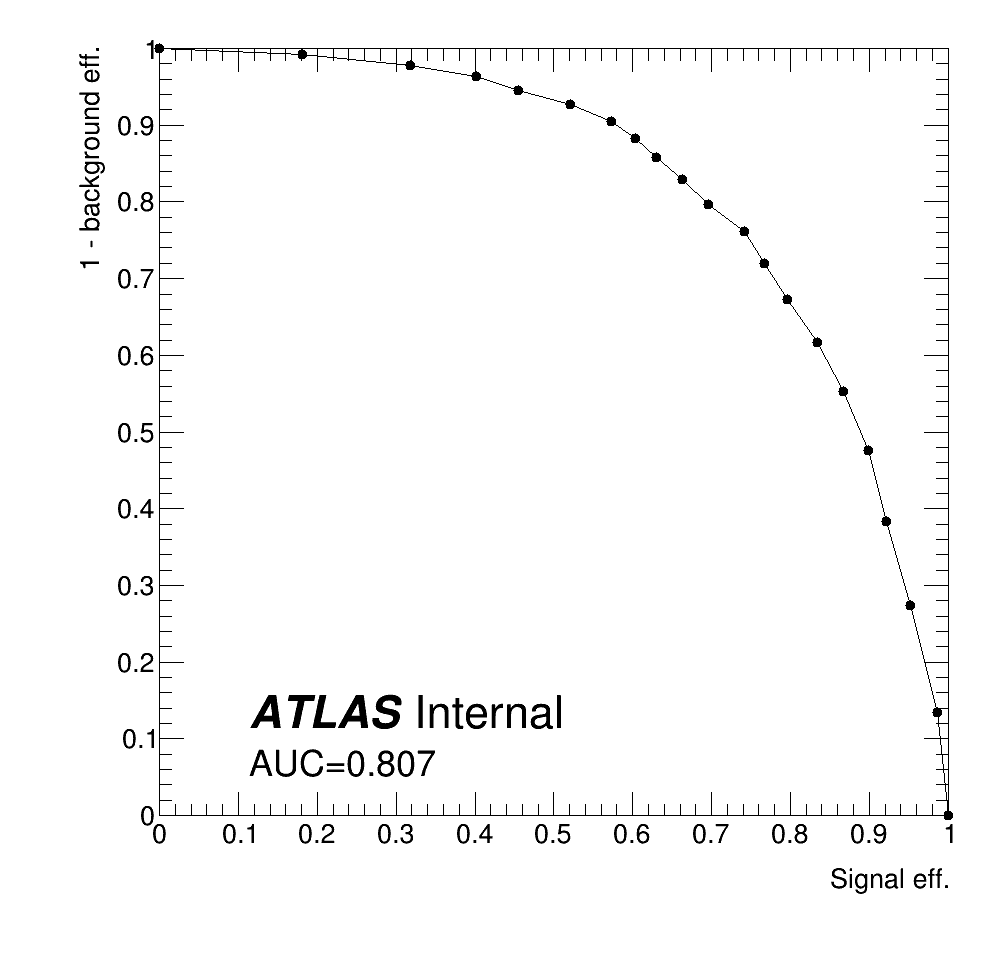
\includegraphics[width=0.45\textwidth]{images/AnalysisStrategy/ROCCurve_Hp1000_Contained80_DL1r_70.png}
    \label{fig:ROCCurve_Hp1000}
  }
  \caption{BDT distribution and ROC curve for the 1000 GeV $H^{+}$ mass hypothesis.}
  \label{fig:BDTTrainingResults_Hp1000}
\end{figure}

\begin{figure}[H]
  \centering
  \subfloat[BDT output]{
    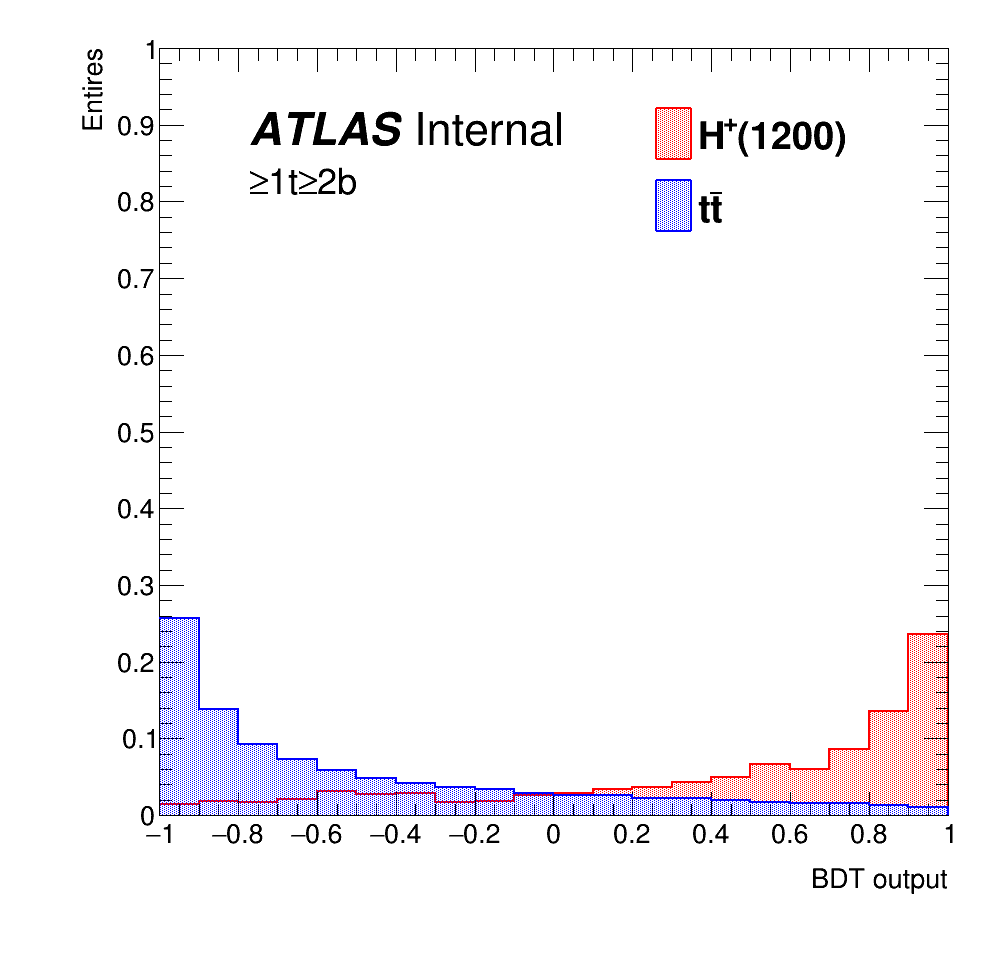
\includegraphics[width=0.45\textwidth]{images/AnalysisStrategy/BDTOutput_Hp1200_Contained80_DL1r_70.png}
    \label{fig:BDTOutput_Hp1200}
  }
  \subfloat[ROC curve]{
    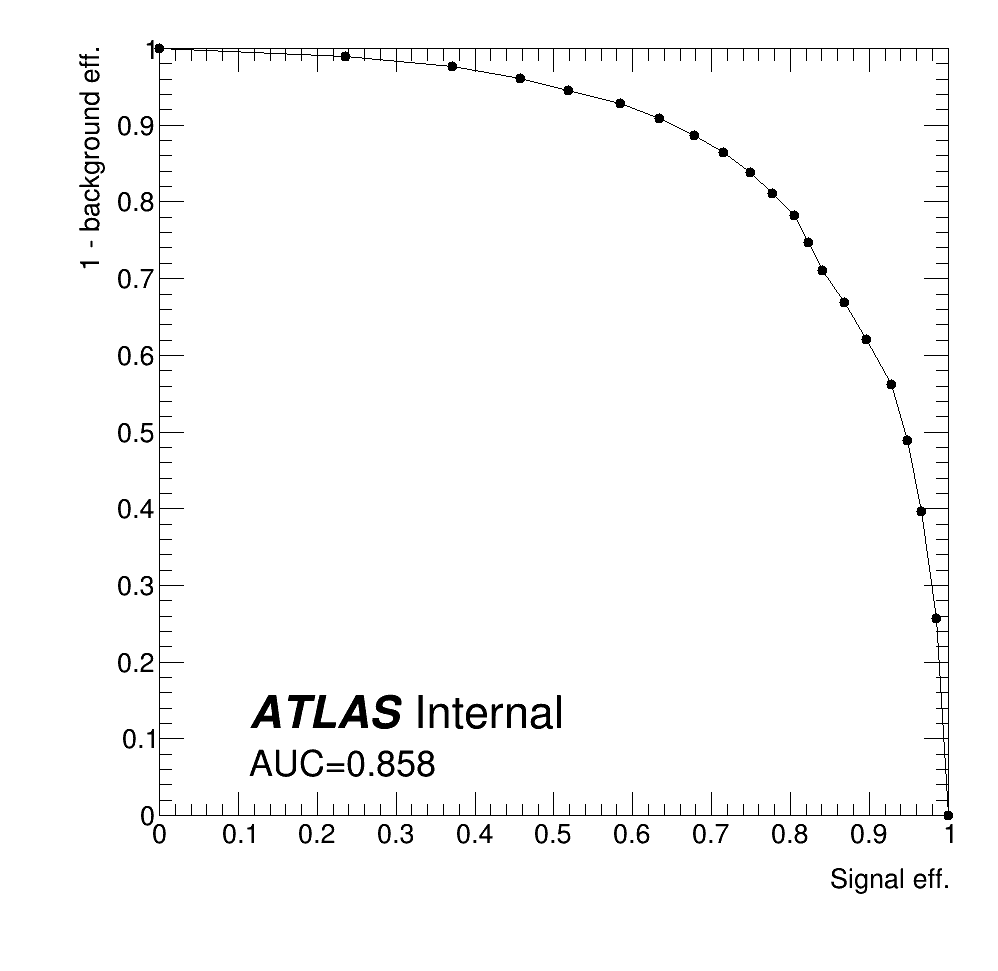
\includegraphics[width=0.45\textwidth]{images/AnalysisStrategy/ROCCurve_Hp1200_Contained80_DL1r_70.png}
    \label{fig:ROCCurve_Hp1200}
  }
  \caption{BDT distribution and ROC curve for the 1200 GeV $H^{+}$ mass hypothesis.}
  \label{fig:BDTTrainingResults_Hp1200}
\end{figure}

\begin{figure}[H]
  \centering
  \subfloat[BDT output]{
    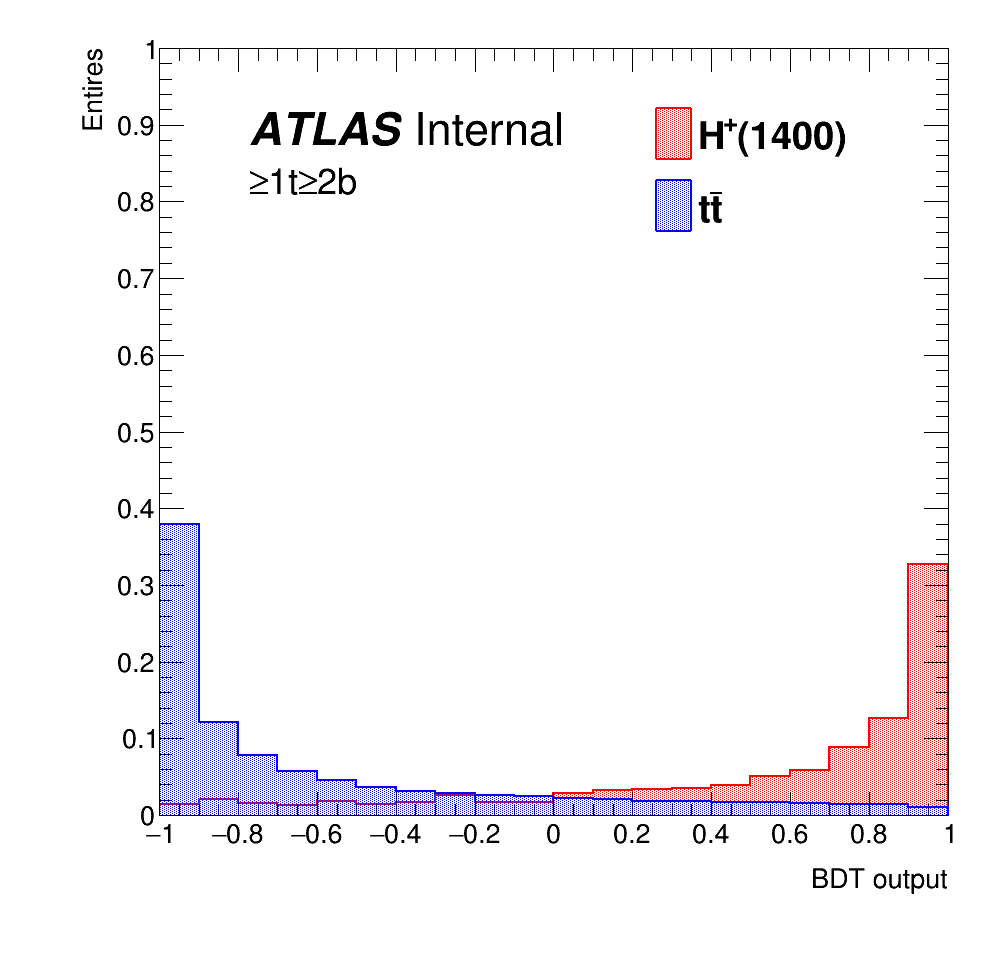
\includegraphics[width=0.45\textwidth]{images/AnalysisStrategy/BDTOutput_Hp1400_Contained80_DL1r_70.png}
    \label{fig:BDTOutput_Hp1400}
  }
  \subfloat[ROC curve]{
    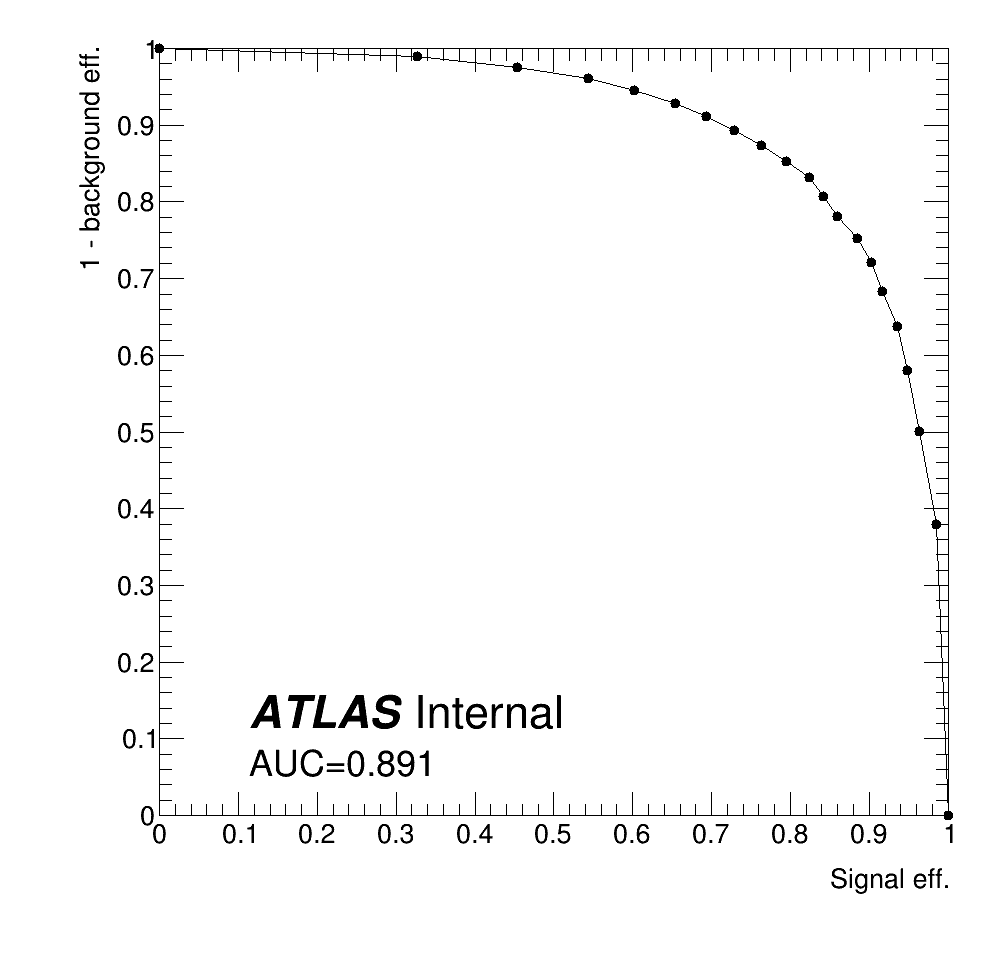
\includegraphics[width=0.45\textwidth]{images/AnalysisStrategy/ROCCurve_Hp1400_Contained80_DL1r_70.png}
    \label{fig:ROCCurve_Hp1400}
  }
  \caption{BDT distribution and ROC curve for the 1400 GeV $H^{+}$ mass hypothesis.}
  \label{fig:BDTTrainingResults_Hp1400}
\end{figure}

\begin{figure}[H]
  \centering
  \subfloat[BDT output]{
    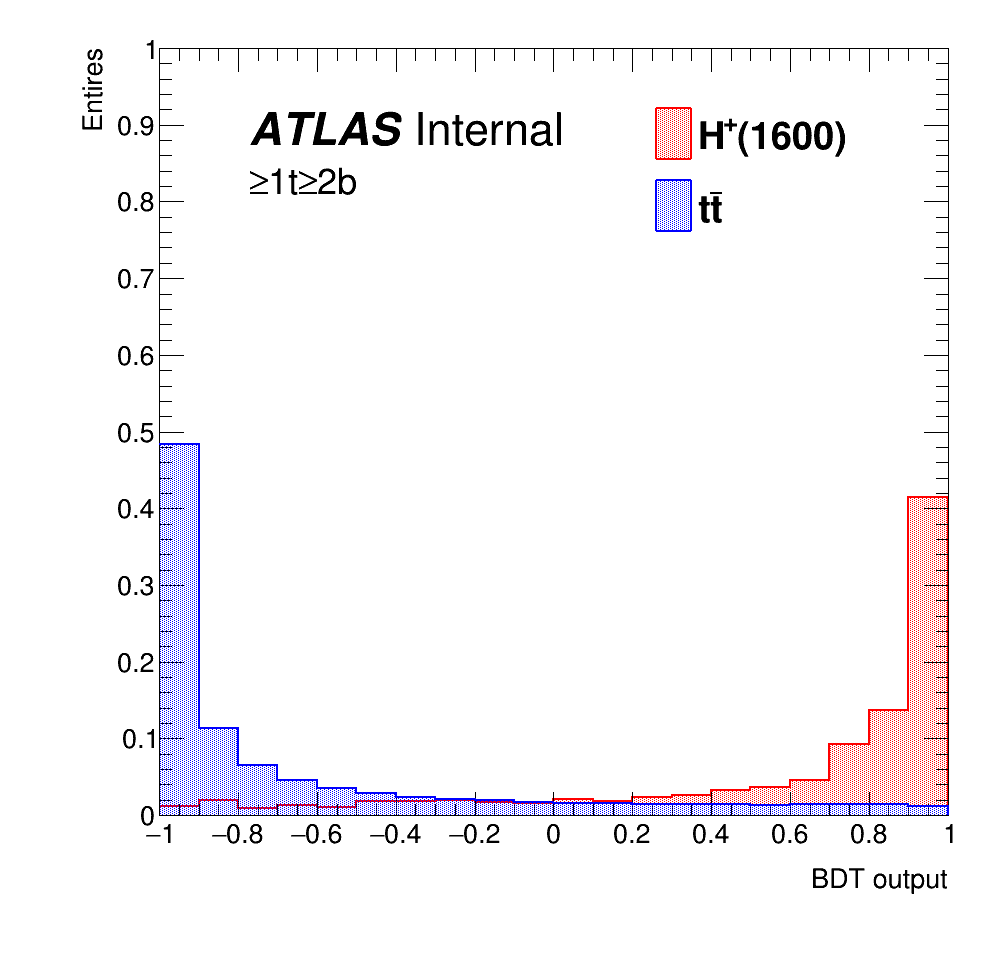
\includegraphics[width=0.45\textwidth]{images/AnalysisStrategy/BDTOutput_Hp1600_Contained80_DL1r_70.png}
    \label{fig:BDTOutput_Hp1600}
  }
  \subfloat[ROC curve]{
    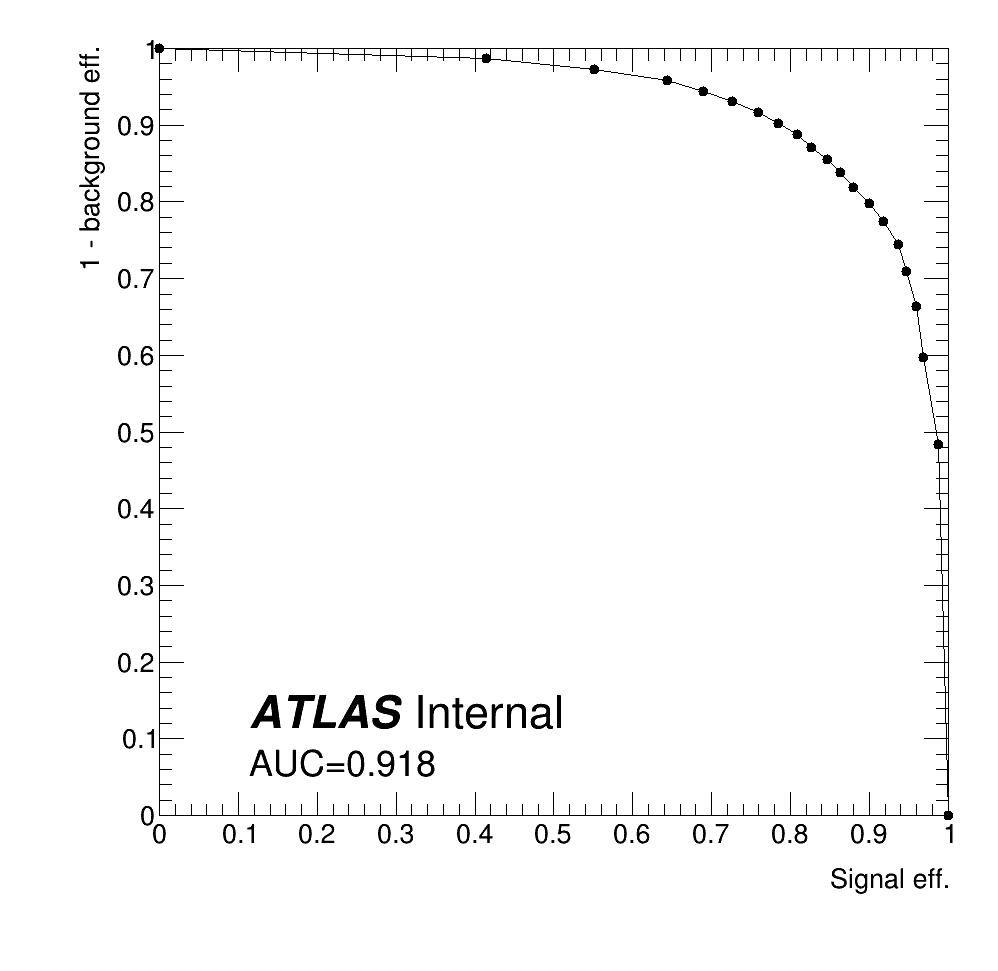
\includegraphics[width=0.45\textwidth]{images/AnalysisStrategy/ROCCurve_Hp1600_Contained80_DL1r_70.png}
    \label{fig:ROCCurve_Hp1600}
  }
  \caption{BDT distribution and ROC curve for the 1600 GeV $H^{+}$ mass hypothesis.}
  \label{fig:BDTTrainingResults_Hp1600}
\end{figure}

\begin{figure}[H]
  \centering
  \subfloat[BDT output]{
    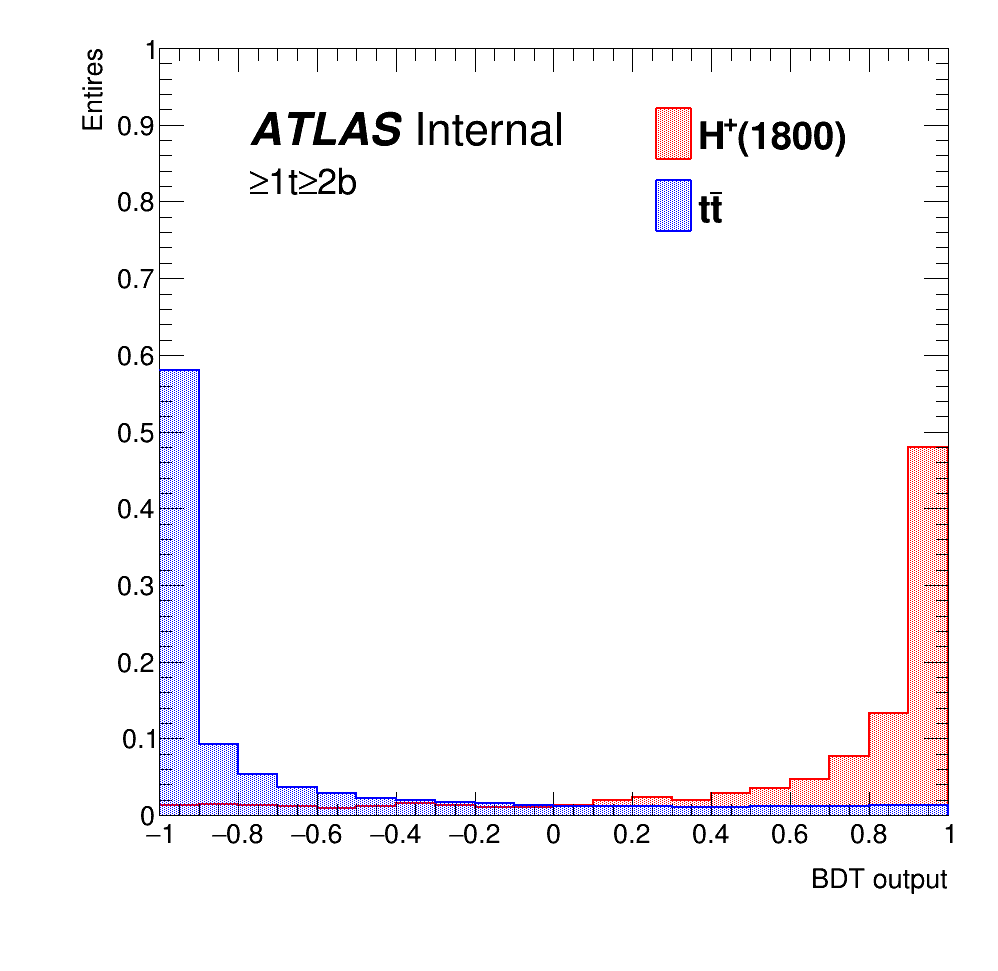
\includegraphics[width=0.45\textwidth]{images/AnalysisStrategy/BDTOutput_Hp1800_Contained80_DL1r_70.png}
    \label{fig:BDTOutput_Hp1800}
  }
  \subfloat[ROC curve]{
    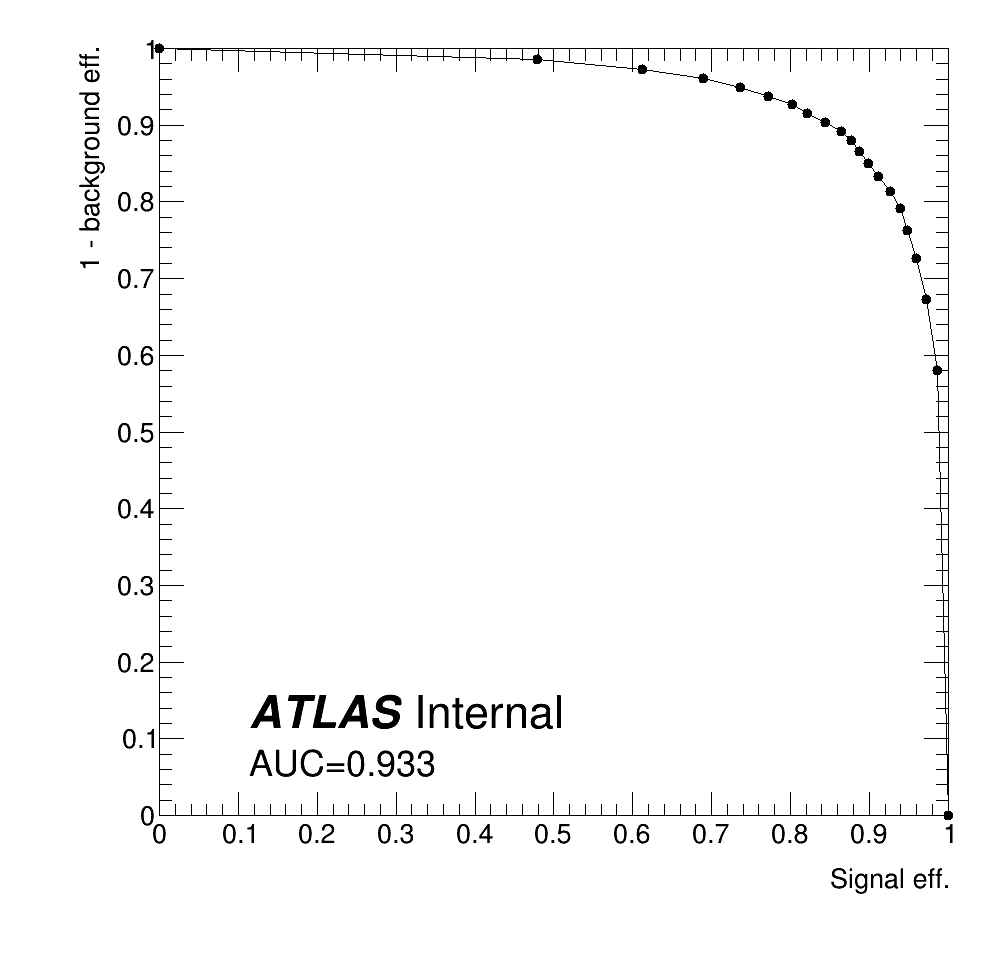
\includegraphics[width=0.45\textwidth]{images/AnalysisStrategy/ROCCurve_Hp1800_Contained80_DL1r_70.png}
    \label{fig:ROCCurve_Hp1800}
  }
  \caption{BDT distribution and ROC curve for the 1800 GeV $H^{+}$ mass hypothesis.}
  \label{fig:BDTTrainingResults_Hp1800}
\end{figure}

\begin{figure}[H]
  \centering
  \subfloat[BDT output]{
    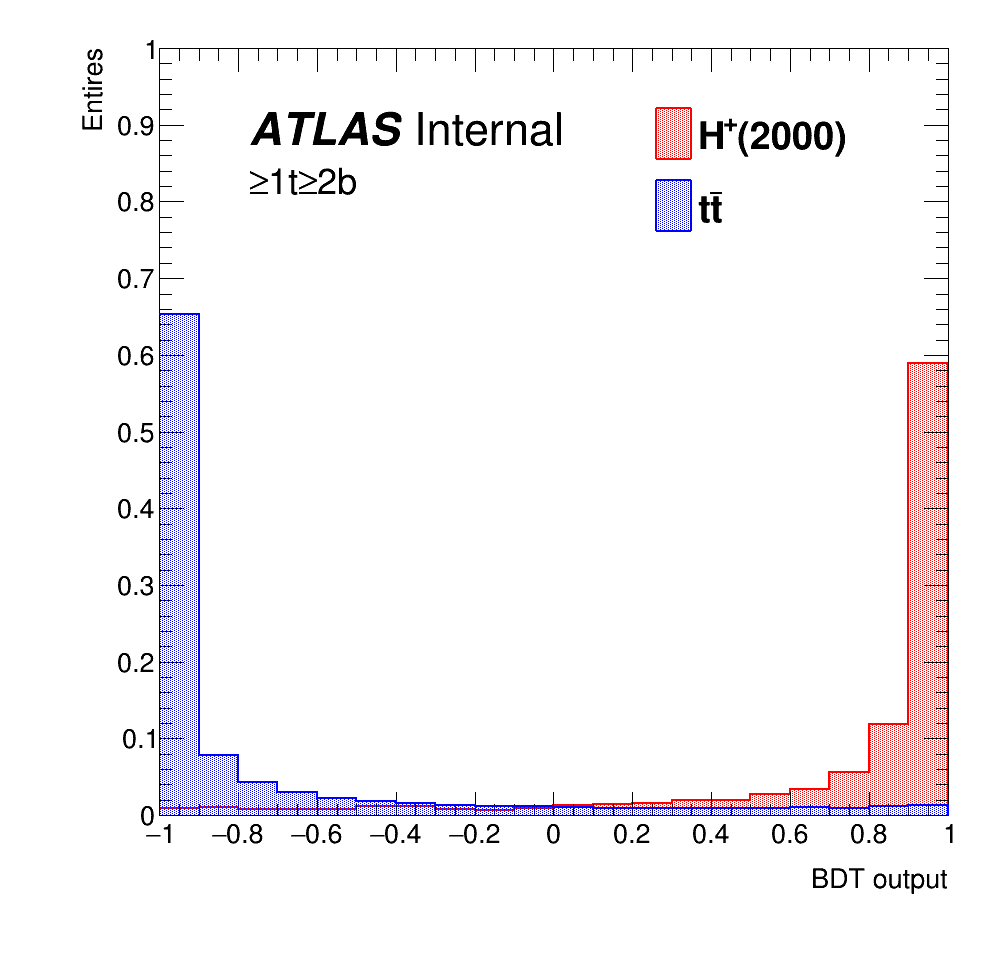
\includegraphics[width=0.45\textwidth]{images/AnalysisStrategy/BDTOutput_Hp2000_Contained80_DL1r_70.png}
    \label{fig:BDTOutput_Hp2000}
  }
  \subfloat[ROC curve]{
    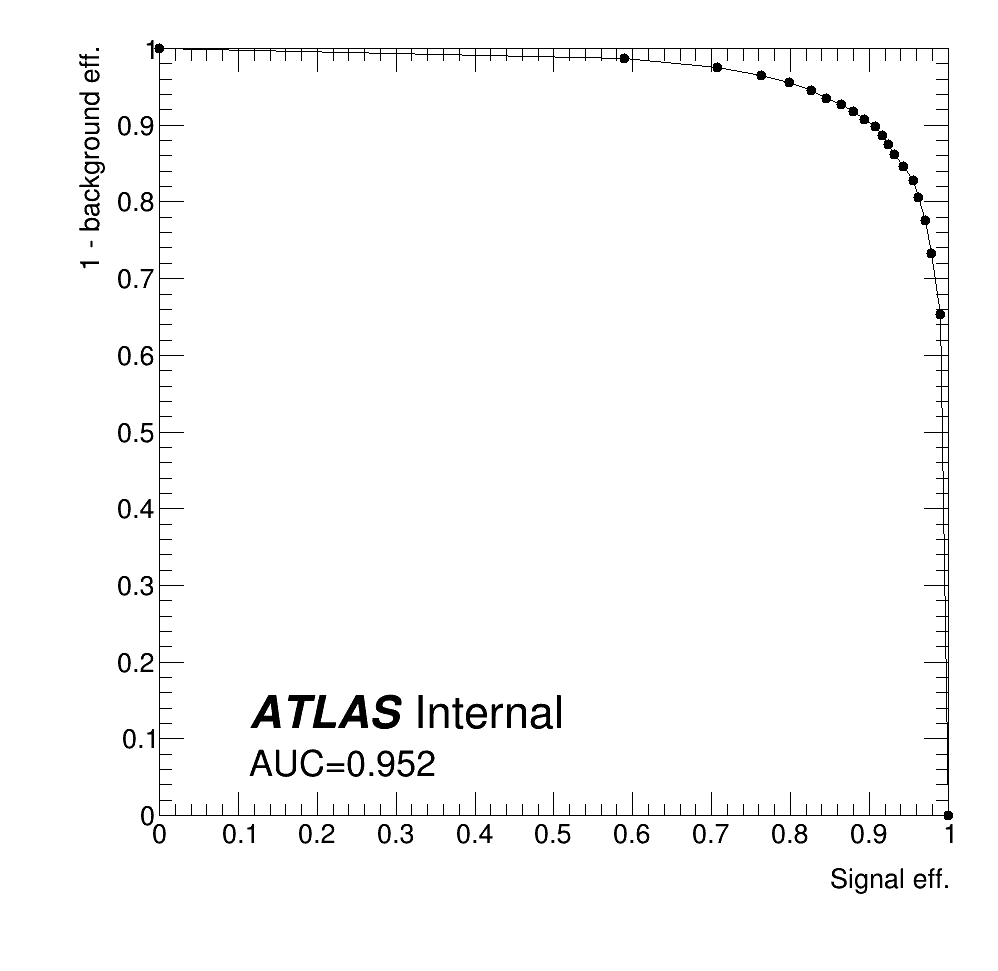
\includegraphics[width=0.45\textwidth]{images/AnalysisStrategy/ROCCurve_Hp2000_Contained80_DL1r_70.png}
    \label{fig:ROCCurve_Hp2000}
  }
  \caption{BDT distribution and ROC curve for the 2000 GeV $H^{+}$ mass hypothesis.}
  \label{fig:BDTTrainingResults_Hp2000}
\end{figure}

\begin{figure}[H]
  \centering
  \subfloat[BDT output]{
    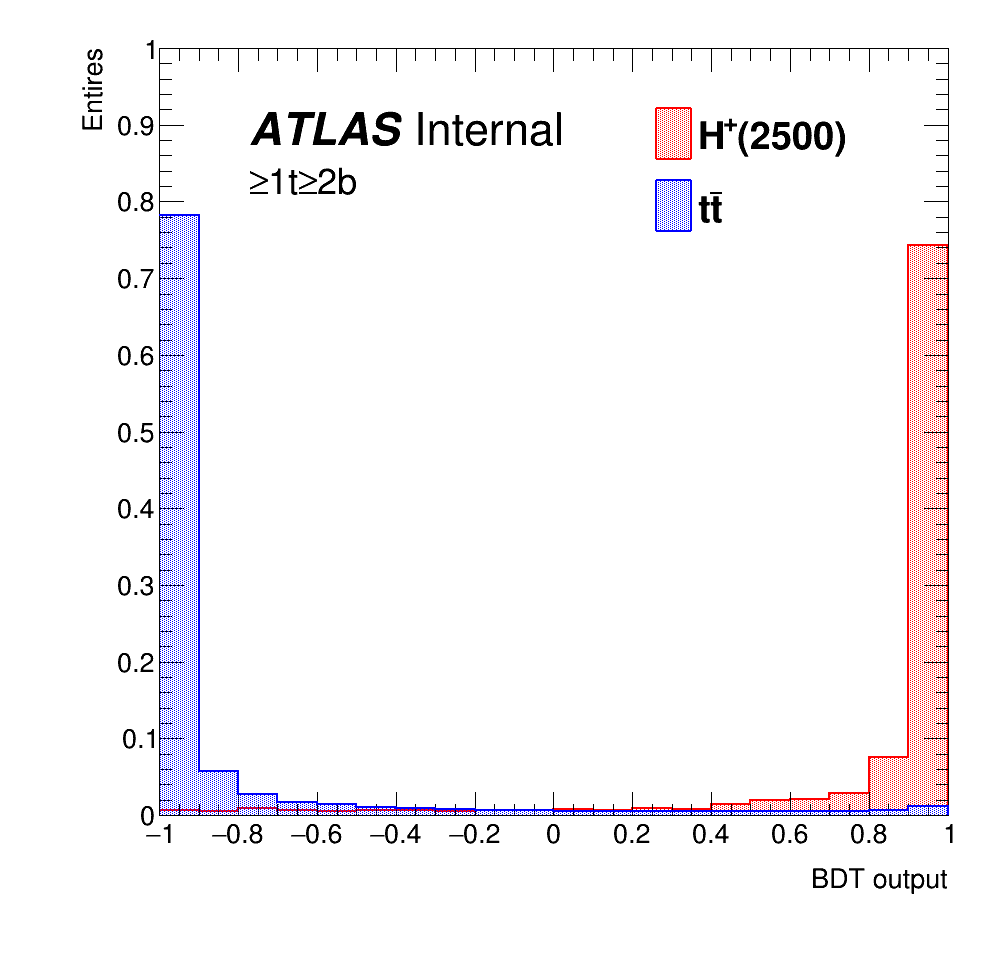
\includegraphics[width=0.45\textwidth]{images/AnalysisStrategy/BDTOutput_Hp2500_Contained80_DL1r_70.png}
    \label{fig:BDTOutput_Hp2500}
  }
  \subfloat[ROC curve]{
    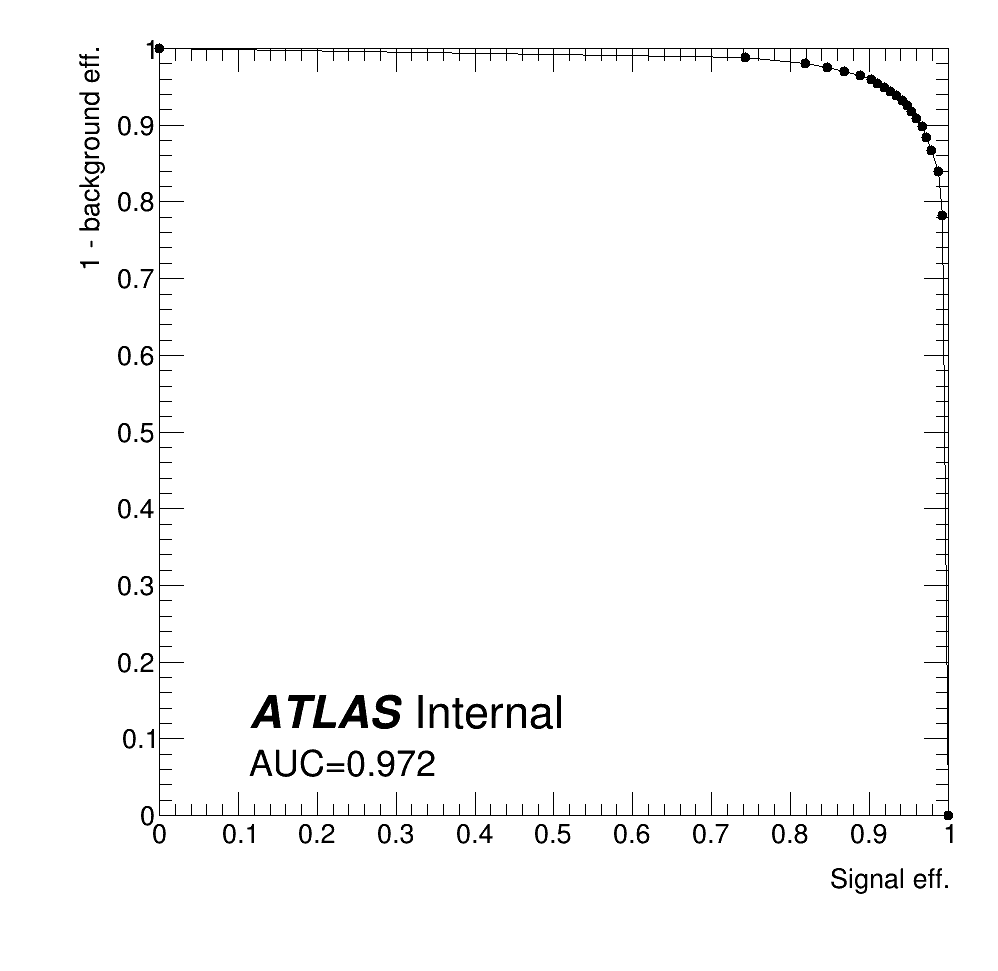
\includegraphics[width=0.45\textwidth]{images/AnalysisStrategy/ROCCurve_Hp2500_Contained80_DL1r_70.png}
    \label{fig:ROCCurve_Hp2500}
  }
  \caption{BDT distribution and ROC curve for the 2500 GeV $H^{+}$ mass hypothesis.}
  \label{fig:BDTTrainingResults_Hp2500}
\end{figure}

\begin{figure}[H]
  \centering
  \subfloat[BDT output]{
    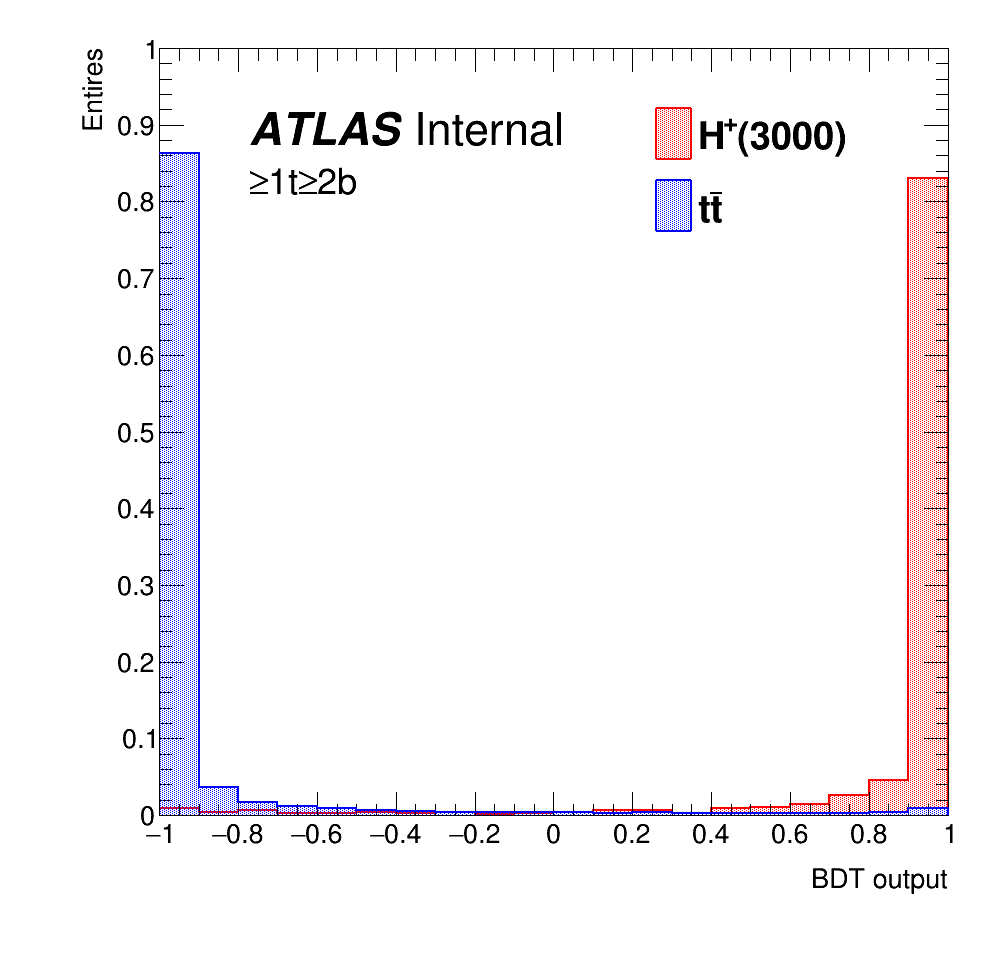
\includegraphics[width=0.45\textwidth]{images/AnalysisStrategy/BDTOutput_Hp3000_Contained80_DL1r_70.png}
    \label{fig:BDTOutput_Hp3000}
  }
  \subfloat[ROC curve]{
    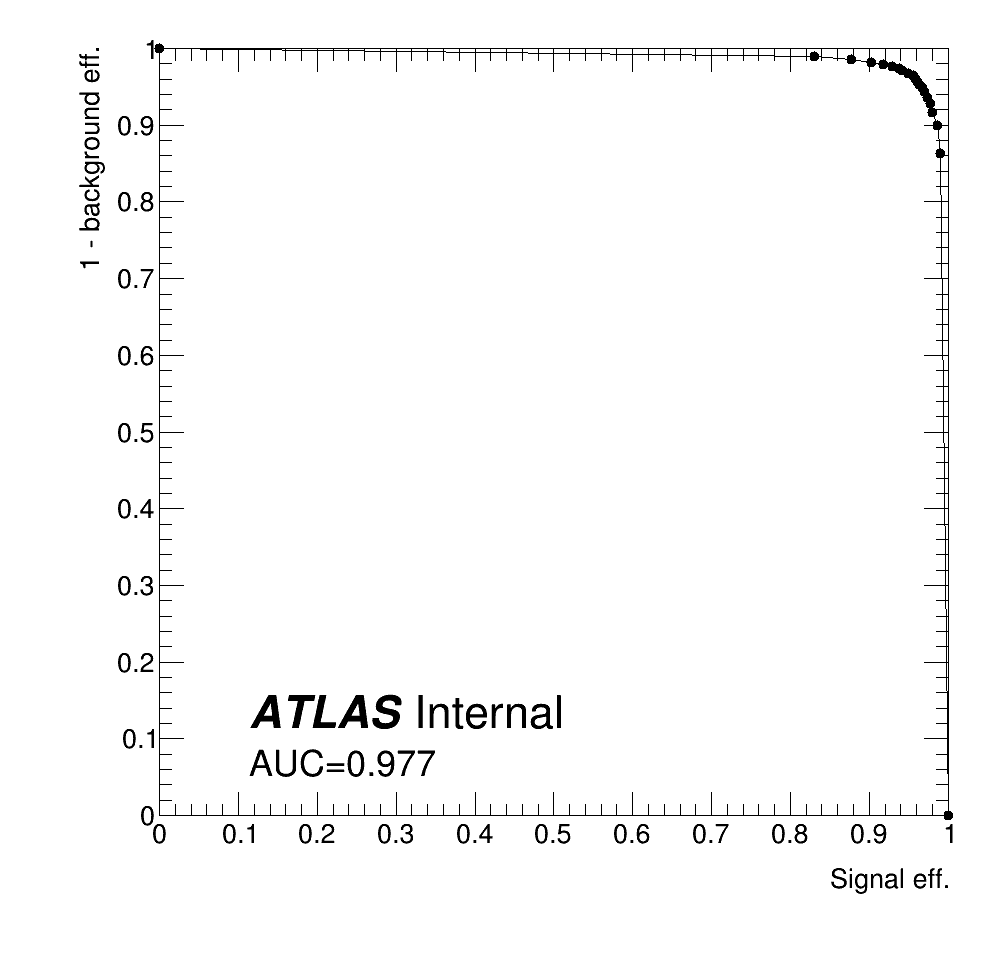
\includegraphics[width=0.45\textwidth]{images/AnalysisStrategy/ROCCurve_Hp3000_Contained80_DL1r_70.png}
    \label{fig:ROCCurve_Hp3000}
  }
  \caption{BDT distribution and ROC curve for the 3000 GeV $H^{+}$ mass hypothesis.}
  \label{fig:BDTTrainingResults_Hp3000}
\end{figure}

\begin{figure}[H]
  \centering
  \subfloat[BDT output]{
    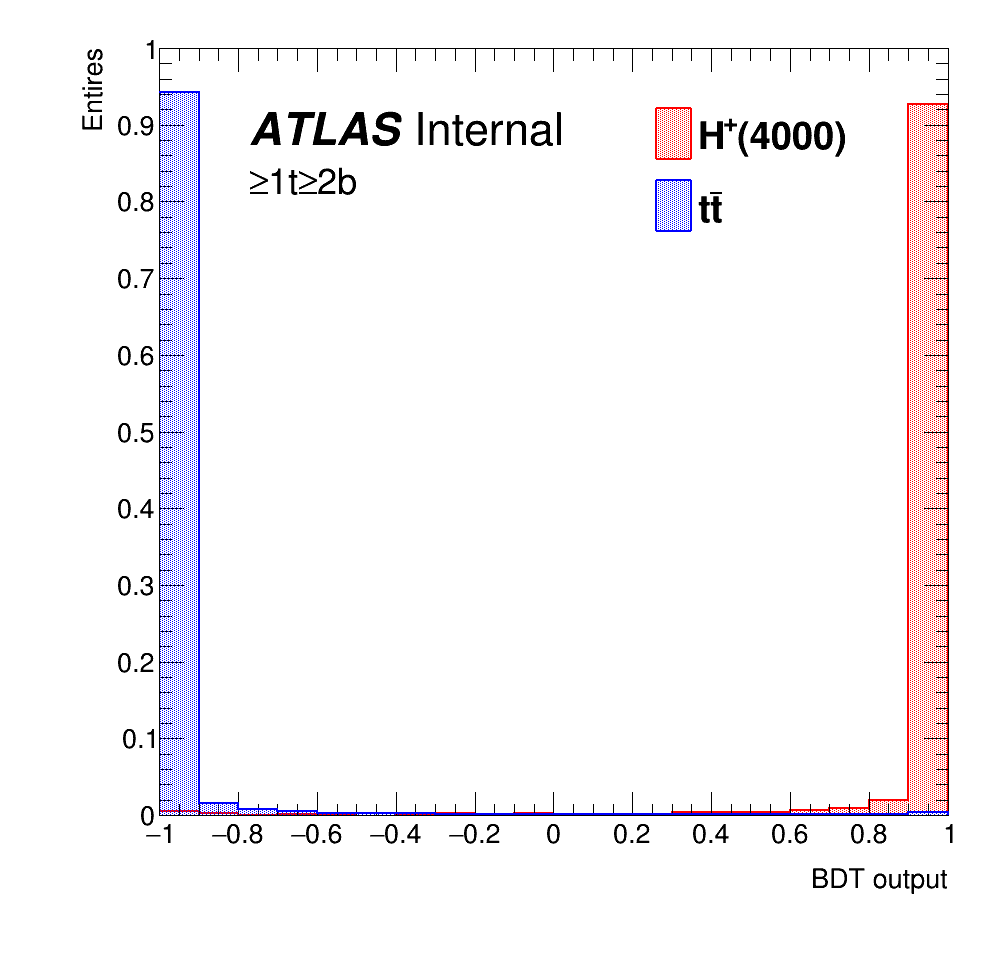
\includegraphics[width=0.45\textwidth]{images/AnalysisStrategy/BDTOutput_Hp4000_Contained80_DL1r_70.png}
    \label{fig:BDTOutput_Hp4000}
  }
  \subfloat[ROC curve]{
    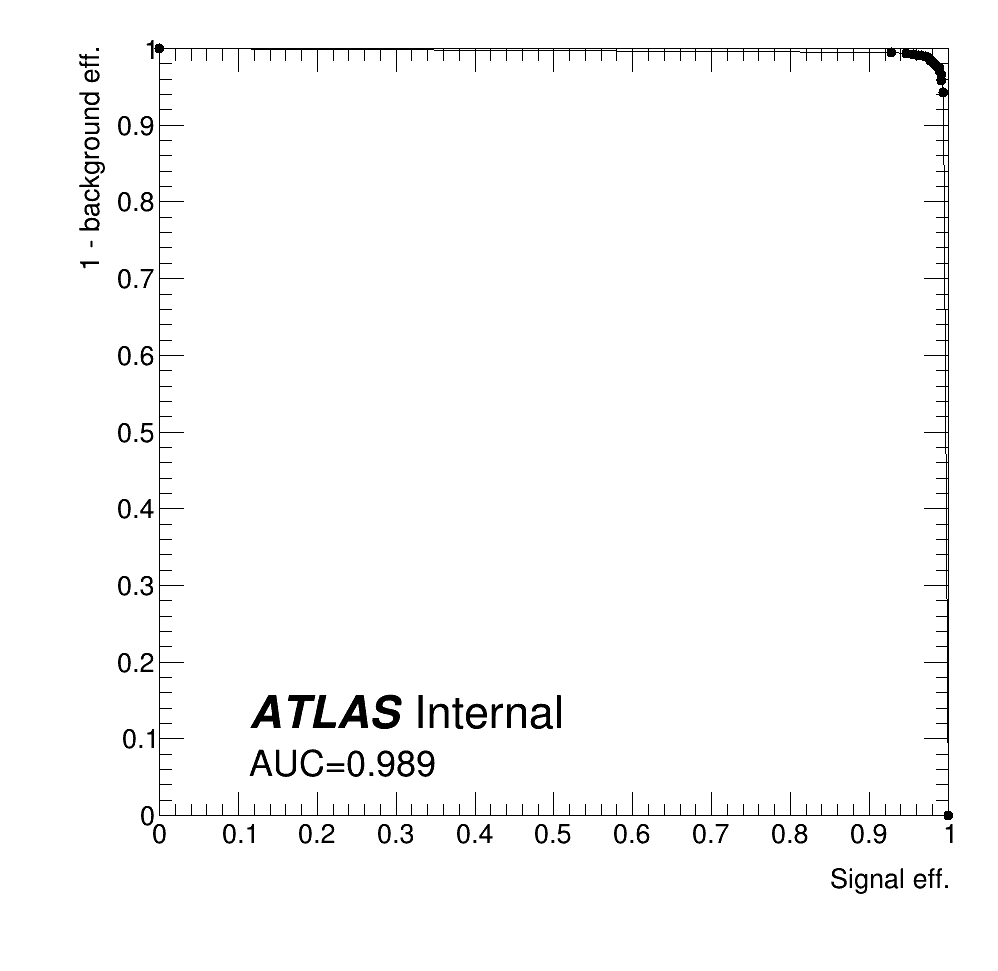
\includegraphics[width=0.45\textwidth]{images/AnalysisStrategy/ROCCurve_Hp4000_Contained80_DL1r_70.png}
    \label{fig:ROCCurve_Hp4000}
  }
  \caption{BDT distribution and ROC curve for the 4000 GeV $H^{+}$ mass hypothesis.}
  \label{fig:BDTTrainingResults_Hp4000}
\end{figure}

\begin{figure}[H]
  \centering
  \subfloat[BDT output]{
    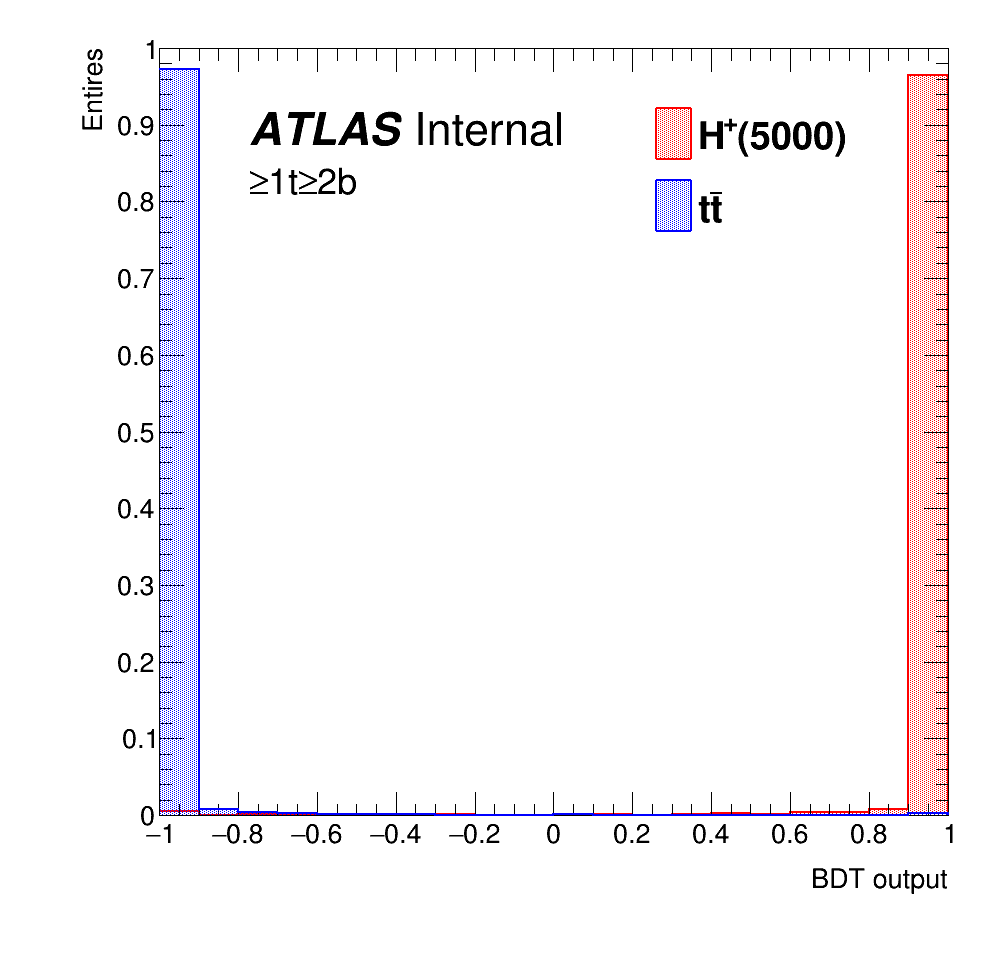
\includegraphics[width=0.45\textwidth]{images/AnalysisStrategy/BDTOutput_Hp5000_Contained80_DL1r_70.png}
    \label{fig:BDTOutput_Hp5000}
  }
  \subfloat[ROC curve]{
    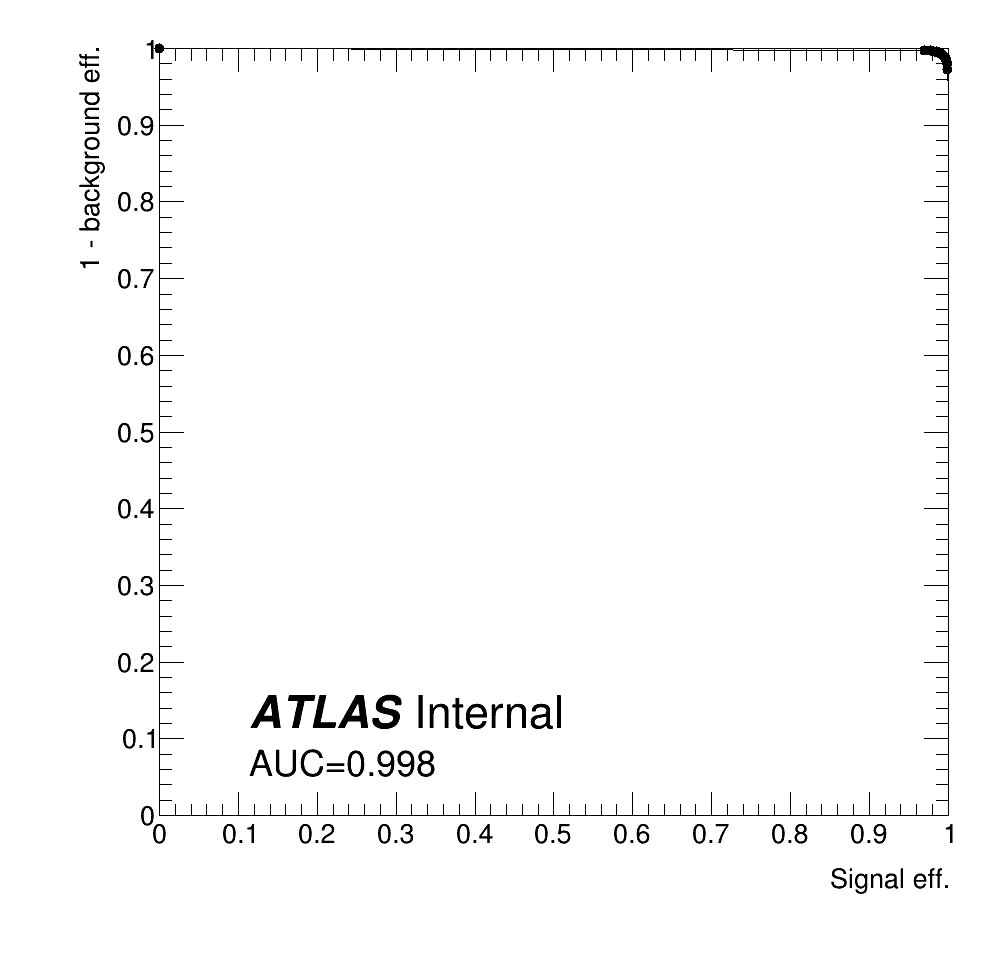
\includegraphics[width=0.45\textwidth]{images/AnalysisStrategy/ROCCurve_Hp5000_Contained80_DL1r_70.png}
    \label{fig:ROCCurve_Hp5000}
  }
  \caption{BDT distribution and ROC curve for the 5000 GeV $H^{+}$ mass hypothesis.}
  \label{fig:BDTTrainingResults_Hp5000}
\end{figure}
